%gji_extra_guide.tex
% \documentclass[extra,mreferee]{gji}
% \usepackage{mathrsfs,amsmath}
% \usepackage{timet}

\documentclass[a4paper, 11pt]{article}
\usepackage[pdftex]{graphicx}
\usepackage{fullpage}
\usepackage{mathrsfs, amsmath, amsfonts}
\usepackage{framed, color, fancybox}

\author{Seogi Kang and Douglas W. Oldenburg}  
\title{On recovering distributed IP information from inductive source time domain electromagnetic data} 


%% =============================================================================
%% My equations
%% =============================================================================

\renewcommand{\div}{\nabla\cdot}
\newcommand{\grad}{\vec \nabla}
\newcommand{\curl}{{\vec \nabla}\times}
\newcommand {\J}{{\vec J}}
\renewcommand{\H}{{\vec H}}
\newcommand {\E}{{\vec E}}
\newcommand{\siginf}{\sigma_\infty}
\newcommand{\dsig}{\triangle\sigma}
\newcommand{\dcurl}{{\mathbf C}}
\newcommand{\dgrad}{{\mathbf G}}
\newcommand{\Acf}{{\mathbf A_c^f}}
\newcommand{\Ace}{{\mathbf A_c^e}}
\renewcommand{\S}{{\mathbf \Sigma}}
\newcommand{\St}{{\mathbf \Sigma_\tau}}
\newcommand{\T}{{\mathbf T}}
\newcommand{\Tt}{{\mathbf T_\tau}}
\newcommand{\diag}{\mathbf{diag}}
\newcommand{\M}{{\mathbf M}}
\newcommand{\MfMui}{{\M^f_{\mu^{-1}}}}
\newcommand{\MfMuoi}{{\M^f_{\mu_0^{-1}}}}
\newcommand{\dMfMuI}{{d_m (\M^f_{\mu^{-1}})^{-1}}}
\newcommand{\dMfMuoI}{{d_m (\M^f_{\mu_0^{-1}})^{-1}}}
\newcommand{\MeSig}{{\M^e_\sigma}}
\newcommand{\MeSigInf}{{\M^e_{\sigma_\infty}}}
\newcommand{\MeSigInfEtab}{{\M^e_{\sigma_\infty \bar{\eta}}}}
\newcommand{\MeSigInfEtat}{{\M^e_{\sigma_\infty \peta}}}
\newcommand{\MedSig}{{\M^e_{\triangle\sigma}}}
\newcommand{\MeSigO}{{\M^e_{\sigma_0}}}
\newcommand{\Me}{{\M^e}}
\newcommand{\Js}{\mathbf{J}^s}
\newcommand{\Mes}[1]{{\M^e_{#1}}}
\newcommand{\Mee}{{\M^e_e}}
\newcommand{\Mej}{{\M^e_j}}
\newcommand{\BigO}[1]{\mathcal{O}\bigl(#1\bigr)}
\newcommand{\bE}{\mathbf{E}}
\newcommand{\bEp}{\mathbf{E}^p}
\newcommand{\bB}{\mathbf{B}}
\newcommand{\bBp}{\mathbf{B}^p}
\newcommand{\bEs}{\mathbf{E}^s}
\newcommand{\bBs}{\mathbf{B}^s}
\newcommand{\bH}{\mathbf{H}}
\newcommand{\B}{\vec{B}}
\newcommand{\D}{\vec{D}}
\renewcommand{\H}{\vec{H}}
\newcommand{\s}{\vec{s}}
\newcommand{\bfJ}{\bf{J}}
\newcommand{\vecm}{\vec m}
\renewcommand{\Re}{\mathsf{Re}}
\renewcommand{\Im}{\mathsf{Im}}
\renewcommand {\j}  { {\vec j} }
\newcommand {\h}  { {\vec h} }
\renewcommand {\b}  { {\vec b} }
\newcommand {\e}  { {\vec e} }
\renewcommand {\d}  { {\vec d} }
\renewcommand {\u}  { {\vec u} }

\renewcommand {\dj}  { {\mathbf{j} } }
\renewcommand {\dh}  { {\mathbf{h} } }
\newcommand {\db}  { {\mathbf{b} } }
\newcommand {\de}  { {\mathbf{e} } }

\newcommand{\vol}{\mathbf{v}}
\newcommand{\I}{\vec{I}}
\newcommand{\A}{\mathbf{A}}
\newcommand{\bI}{\mathbf{I}}
\newcommand{\bus}{\mathbf{u}^s}
\newcommand{\brhss}{\mathbf{rhs}_s}
\newcommand{\bup}{\mathbf{u}^p}
\newcommand{\brhs}{\mathbf{rhs}}
%%-------------------------------
\newcommand{\bon}{b^{on}(t)}
\newcommand{\bp}{b^{p}}
\newcommand{\dbondt}{\frac{db^{on}(t)}{dt}}
\newcommand{\dfdt}{\frac{df(t)}{dt}}
\newcommand{\dfdtdsiginf}{\frac{\partial\frac{df(t)}{dt}}{\partial\siginf}}
\newcommand{\dfdsiginf}{\frac{\partial f(t)}{\partial\siginf}}
\newcommand{\dbgdsiginf}{\frac{\partial b^{Impulse}(t)}{\partial\siginf}}
\newcommand{\digint}{\frac{2}{\pi}\int_0^{\infty}}
\newcommand{\Gbiot}{\mathbf{G}_{Biot}}
%%-------------------------------
\newcommand{\peta}{\tilde{\eta}}
\newcommand{\eFmax}{\e^{\ F}_{max}}
\newcommand{\eref}{\e^{\ ref}}
\newcommand{\jref}{\j^{\ ref}}
\newcommand{\dip}{d^{IP}}
\newcommand{\sigpert}{\delta\sigma}
\newcommand{\bzip}{b_z^{IP}}
\newcommand{\dbzdtip}{\frac{\partial b_z^{IP}}{\partial t}}

%% =============================================================================
%% End of my equations
%% =============================================================================


% \title[] {On recovering distributed IP information in airborne time domain electromagnetic data} 
% \author[] {Seogi Kang and Douglas W. Oldenburg}  
% \newcommand{\btx}{\textsc{BibTeX}}

\begin{document}
\maketitle
\tableofcontents
\clearpage

\section{Introduction}
The electrical conductivity of earth materials can be frequency dependent with the effective conductivity decreasing with decreasing frequency due to the buildup of electric charges that occur under the application of an electric field.
Effectively, the rock is electrically polarized. 
Application of this induced polairzation (IP) technique has been particularly successful in mineral exploration for disseminated sulphide or porphyry deposits (CITES). Sucesses of the IP technique are has been shown in geotechnical and enviromental problems as well (CITES). 
% Finding this induced polarization (IP) response has been important in mineral exploration but it is also important in environmental problems, groundwater flow, and site characterization (CITES). 
Polarization charges can accumulate whenever there is an electric field in a medium. In controlled source surveys, the transmitter can be a galvanic source (a generator attached to two grounded electrodes), or an inductive source (arising from current flowing in a wire loop). Most of the researches and applications have focused upon using grounded electrodes and measuring electric fields (EIP survey)  (\cite{seigel1959}).   Magnetic fields arising from polarization currents (MIP survey) have also been successfully used, particularly in mineral exploration geologies characterized by a conductive overburden (cites). In recent years attention has also turned towards the use of inductive sources. (reasons:  resistive overburden difficult to put current into the ground; also for airborne surveys there is no choice).  Inductive source IP (ISIP),  can have transmitters in the air or on the ground and the waveforms can be in either the frequency or time domain. Recently  (\cite{Marchant2012b}) showed how, by collecting data at two frequencies, it was possible to measure a datum that depended purely on IP signals and that these data can be inverted to recover a 3D distribution of chargeability. 
For time domain systems the observations of negative transients in coincident loop systems provide an distinctive verification of chargeable material (\cite{Weidelt1982}). The negative transients have been frequently observed (CITES; Klein and Smith and a host of others). Effects of chargeable body on this system has been carefully investigated (\cite{Smith1988a,Flis1989,ElKaliouby2004, Kratzer2012,Marchant2014}). 

Extracting information about the complex conductivity can be done in a variety of ways. In principle it can be solved by finding a function $\sigma(x,y,z,\omega)$ or parameterizing the complex conductivity, usually with a Cole-Cole type model, and finding the distribution of those parameters(CITES). Traditionally, however, with EIP and time domain waveforms, one first estimates the background conductivity from the asymptotic on-time data and then inverts off-time data to recover information about ``chargeability'' (\cite{doug1994}) This is carried out by solving a linear inverse problem where the sensitivities depend upon geometry of the survey and the background conductivity. The recovered values are really pseudo-chargeability, and they have the same units as the data (eg. msec, mV/V). The same procedure can be used in frequency domain experiments but the data might have units or mrad, pfe (percent frequency effect). Inversion of IP data to recover 2D or 3D distributions of pseudo-chargeability are now commonly carried out. These inversions delineate locations of high pseudo-chargeability and the geometry of the bodies. MIP data can be inverted with the same methodology (\cite{Chen2003}). 

The physical mechanisms by which polarization charges and currents are established in the ground are independent of their type of transmitter and waveform; the important quantity is the time history of the electric field within the earth. The challenge posed by the use of  inductive sources is that steady state electric fields are not established inside the earth as they are for EIP or MIP surveys. The electric field at any location will increase to a maximum value and then decrease as the EM wave diffuses through. The EM fields at any position and time depend upon the convolution of the electric field with the time-dependent conductivity of the rock. Unravelling these complexities, and providing a framework for extracting information about IP characteristics of rocks, are issues we address in our paper. 

Our procedure involves three principal steps: 1) estimating the 3D background conductivity, 2) carrying out an EM decoupling to produce IP data ($\dip$), and 3) inverting $\dip$ using a linearized kernel  function. Each of these steps requires special attention for inductive source data and approximations are required in order to proceed. We address these as they are encountered. Our paper proceeds as follows. We first outline our decomposition process for obtaining our $\dip$ data, define a pseudo-chargeability, and  show how our problem can be linearized. For ATEM surveys  with multiple transmitters, we show how to generate a single linear inverse problem that can be solved for an approximate pseudo-chargeability. The data and  pseudo-chargeability are linearly related through the Biot-Savart law and hence a depth weighting, required for other potential field inversions, is required to obtain geologic solutions. The inversion can be carried out at multiple times and a pseudo-chargeability as function of time can be generated. These results can be used to recover intrinsic decays of the chargeable rock units and thus potentially differentiate between rock types in the same manner as carried out by \cite{Yuval1997} using EIP data. In our numerical experiments, we investigate the above steps and procedures, test our assumptions, and evaluate the circumstances under which our technique might provide meaningful results. Although  we focus upon airborne TEM data, the analysis we present here is valid for surveys on the earth’s surface using inductive sources and also for grounded sources although many of the complications we deal with are not relevant. 
    
%% =============================================================================
%% Section. Complex conductivity
%% =============================================================================

\section{Complex conductivity}
An often-used representation for complex conductivity in the frequency domain is the Cole-Cole model \cite{COLE}:
\begin{equation}
  \sigma(\omega) = \sigma_{\infty} - \sigma_{\infty}\frac{\eta}{1+(1-\eta)(\imath\omega\tau)^c} = \sigma_{\infty} + \triangle\sigma(\omega),
  \label{eq: sigma_freq}
\end{equation}
where $\sigma_{\infty}$ is the conductivity at infinite frequency, $\eta$ is the intrinsic chareability, $\tau$ is the time constant and $c$ is the frequency dependency. Real and imaginary parts of complex conductivity in frequency domain are shown in Figure ~\ref{Fig:FDandTDCole}(a) with Cole-Cole parameters: $\siginf$ = $10^{-2}$ S/m, $\eta $ = 0.5, $\tau$ = 0.01, and $c$=1. By applying inverse Fourier transform with time dependency, $e^{\imath\omega t}$, we have
\begin{equation}
  \sigma(t) = \mathscr{F}^{-1}[\sigma(\omega)] = \sigma_{\infty}\delta(t) + \triangle\sigma(t)u(t),
  \label{eq: sigma_time}
\end{equation}
where $\delta(t)$ is Dirac delta function, $u(t)$ is Heaviside step function, and $\mathscr{F}^{-1}[\cdot]$ is inverse Fourier transform operator. 
We rewrite $\dsig(t)$ as 
\begin{equation}
  \dsig(t) = - \siginf\peta^{I}(t),
  \label{eq: sigma_time_c1}
\end{equation}
where intrinsic pseudo-chargeability, $\peta^{I}(t)$ is defined as
\begin{equation}
    \peta^{I}(t) = -\frac{\dsig(t)}{\siginf}. %=\frac{\eta}{(1-\eta)\tau}e^{-\frac{t}{(1-\eta)\tau}}u(t)
    \label{eq: intrinsic_peta}
\end{equation}
Cole-Cole model in time domain is also shown in Figure ~\ref{Fig:FDandTDCole}(b). Used Cole-Cole parameters here are same as the above.

\begin{figure}
  \centering
  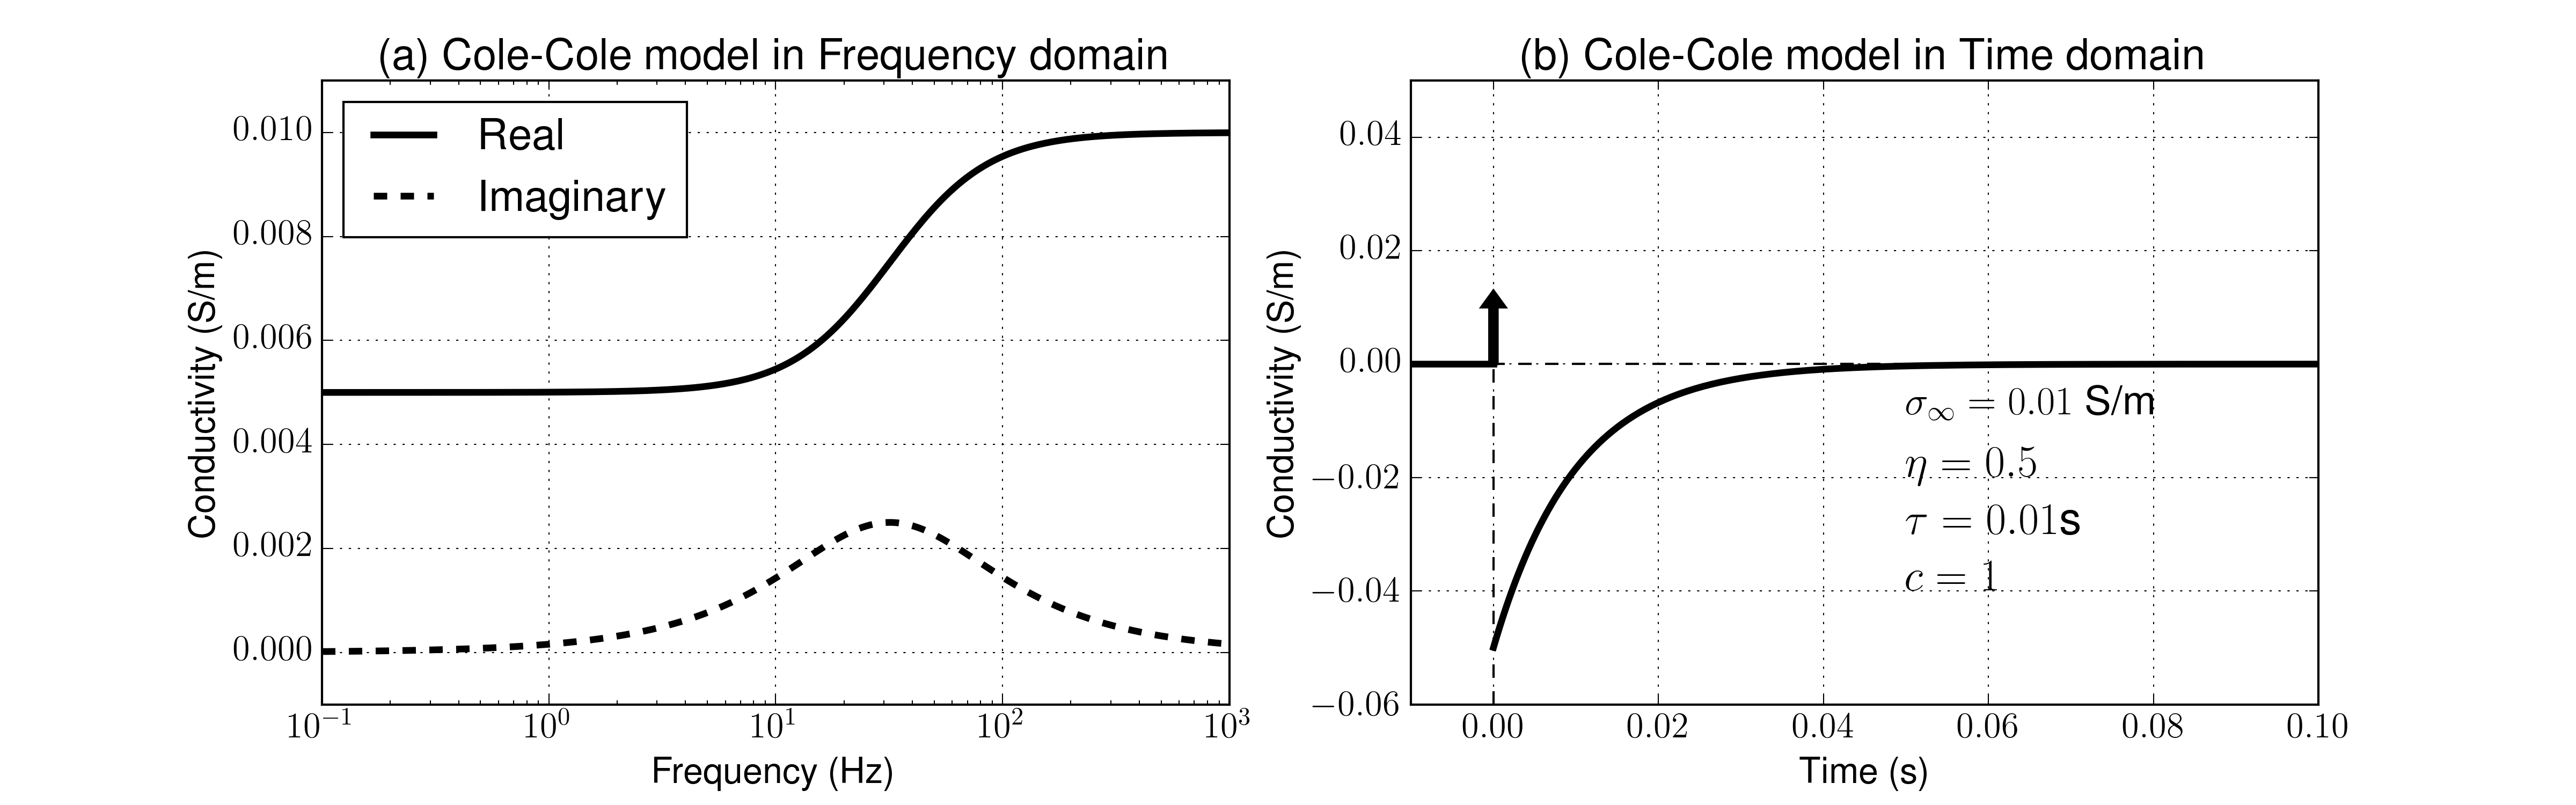
\includegraphics[width=1.0\textwidth]{figures/FDandTDCole.png}
  \caption{Cole-Cole model in frequency domain (a) and time (b) domain. Used Cole-Cole parameters are $\siginf$ = $10^{-2}$ S/m, $\eta $ = 0.5, $\tau$ = 0.01, and $c$=1.}
  \label{Fig:FDandTDCole}
\end{figure}

%% =============================================================================
%% Section. Decomposition of observed responses
%% =============================================================================

\section{Decomposition of observed responses}
IP effects in the observed data are coupled with EM effects. We need to decompose these effects in the observation to isolate only data associated with the IP phenomena.  
Maxwell's equations in time domain with a quasi-static approximation are written as:
\begin{equation}
  \curl{\e} = -\frac{\partial \b}{\partial t},
  \label{eq: total_farad}
\end{equation}
\begin{equation}
  \curl{\frac{1}{\mu}\b} - \j= \j_{s},
  \label{eq: total_coulomb}
\end{equation}
where $\e$ is the electric field ($V/m$), $\b$ is the magnetic flux density ($Wb/m^2$) and $\mu$ is the magnetic permeability ($H/m$). Here $\j$ is the conduction current. In the frequency domain, this conduction current, $\J$ is related to conductivity via Ohm’s law: $\J(\omega) = \sigma(\omega)\E(\omega)$ where $\E$ is the electric field. 
Converting this relationship to time domain using the inverse Fourier transform yields:
\begin{equation}
  \j(t) = \sigma(t)\otimes \e(t) = \int_0^t \sigma(u) e(t-u) du.
  \label{eq: ohms_law_convolution}
\end{equation}
where $\otimes$ indicates time convolution for a causal signal.  
Thus the current density depends upon the previous history of the electric field.
As in \cite{Smith1988a}, we let total fields as $\e = \e^{F} + \e^{IP}$, $\b = \b^{F} + \b^{IP}$ and $\j = \j^{F} + \j^{IP}$, where superscript $F$ indicates fundamental and $IP$ is induced polarization. 
Here fundamental fields indicate EM fields without IP effects. 
Substituting into equations (\ref{eq: total_farad}) and (\ref{eq: total_coulomb}) yields the following sequences:
\begin{equation}
  \curl({\e^{F}+\e^{IP}}) = -\frac{\partial}{\partial t} (\b^{F}+\b^{IP}),
\end{equation}
\begin{equation}
  \curl\frac{1}{\mu}(\b^{F}+\b^{IP}) - (\j^{F}+\j^{IP})= \j_{s}.
\end{equation}

The fundmental equations can be written as
\begin{equation}
  \curl \e^{F} = -\frac{\partial \b^{F}}{\partial t},
  \label{eq: eq_primary_farad}
\end{equation}
\begin{equation}
  \curl{\frac{1}{\mu}\b^{F}} -\j^{F} = \j_s.
  \label{eq: eq_primary_coulomb}
\end{equation}
Here
\begin{equation}
  \j^{F} = \siginf\e^{F}.
  \label{eq: jF}
\end{equation}

Substituting the fundamental fields into equations (\ref{eq: total_farad}) and (\ref{eq: total_coulomb}) yields the expressions for the IP fields 
\begin{equation}
  \curl \e^{IP} = -\frac{\partial \b^{IP}}{\partial t},
  \label{eq: eq_secondary_farad}
\end{equation}
\begin{equation}
  \curl{\frac{1}{\mu}\b^{IP}} = \j^{IP}.
  \label{eq: eq_secondary_coulomb}
\end{equation}

Let $F[\cdot]$ denote operator associated with Maxwell’s equations, and let $d$ denote the observations that include both EM and IP effects. 
Keeping the same notation, we can obtain $d = d^{F} + \dip$, where $d^F$ and $\dip$ are fundamental and IP responses, respectively. 
Based on this, we define the IP datum as 
\begin{equation}
  \dip = d - d^{F} = F[\sigma(t)]-F[\siginf].
    \label{eq: IPdatum_syn}
\end{equation}
Here $F[\siginf]$ corresponds to the fundamental response ($d^F$). 
This subtraction process acts as an EM decoupling process, which removes the EM effects from the measured responses. This is the same procedure that formed the basis of work by \cite{routh2001}. 

%% ============================================================
%% Section. Pseudo-chargeability for inductive sources
%% ============================================================
\section{Pseudo-chargeability for inductive sources}
%% later
% A major difference of the inductive source from the galvanic source is the absence of the steady-state electric field. 
% This generates a principal difference on the IP response for both inductive and galvanic sources. 
% To examine this, we define the IP current ($\j^{IP}$) as
Combining equations (\ref{eq: sigma_time}) and  (\ref{eq: ohms_law_convolution}) writing $j(t)=j^F + j^{IP}$ we obtain
\begin{equation}
  \j^{IP} = \siginf \e^{IP} + \j^{pol},
  \label{eq:IP_current}
\end{equation}
where the polarization current ($\j^{pol}$) is
\begin{equation}
  \j^{pol}(t) = \dsig(t)u(t) \otimes \e(t).
  \label{eq:polarization_current}
\end{equation}

If the electric field has different characteristics for the inductive and galvanic sources and this will generate different features in the polarization current.  
We consider two cases: a) galvanic source without EM induction and b) inductive source with EM induction. The first case corresponds to EIP (\cite{seigel1959}), and the second one is ISIP.
Figure \ref{F:DCEM_F_current} shows the amplitude of the fundamental electric field ($\e^{F}$) in the earth for those two cases. 
For the galvanic source, the electric field is instantaneous due to the steady-state electric field (Figure \ref{F:DCEM_F_current} (a)). 
However, for the inductive source, the electric field in the off-time is not zero, but increases to a peak and then decays as shown in Figure \ref{F:DCEM_F_current} (b). 
The polarization current for the two different sources will be significantly affected by these different electric fields. 
To capture this difference in a linearized kernel for the IP response, we define pseudo-chargeability ($\peta(t)$) as 
\begin{equation}
  \peta(t) = -\frac{\j^{pol}(t)}{\j^{\ ref}},
  \label{eq:pseudochargeability_0}
\end{equation}
where the reference current ($\j^{ref}$) is defined as 
\begin{equation}
  \j^{\ ref} = \siginf \eref.
  \label{eq:reference_current}
\end{equation}
Here $\eref$ is the reference electric field and both $\j^{\ ref}$ and $\eref$ are static fields that are independent of time. 
The pseudo-chargeability defined in equation (\ref{eq:pseudochargeability_0})  is the ratio of  the polarization current to the reference current. This is a small quantity and it plays an essential role in our linearization. 

To evaluate the pseudo-chargeability, we have to identify the reference current or reference electric fields. For the EIP case, the electric field, when there is no IP present, is independent of time as shown in Figure \ref{F:DCEM_F_current}(a) and any on-time value of the field can serve as a reference. For the inductive source however, the electric field does not achieve a steady-state, but increases to the peak then decreases. Our choice of the reference electric field is the maximum of the $\e^{F}$ and the  time at which the  maximum electric field occurs is our reference time ($t^{\ ref}$).
Each pixel in the Earth has its own reference electric field and time thus  both $\eref$ and $t^{\ ref}$ have a 3D distribution. 
For both EIP and ISIP cases, we mathematically present our choice of the reference electric field as
\begin{equation}
  \eref = \e^{F}(t) \otimes \delta(t-t^{\ ref}). 
  \label{eq:reference_electricfield}
\end{equation}
The reference time for the EIP case can be any time in the on-time, because the fundamental electric field for the EIP case does not change in on-time. 

By rearranging equation (\ref{eq:pseudochargeability_0}), we obtain 
\begin{equation}
  \j^{pol} = -\jref\peta(t). 
  \label{eq:polarization_current_concept}
\end{equation}
This states that the polarization current has an opposite direction to the reference current, and is proportional to the pseudo-chargeability ($\peta(t)$). 
This conceptual model about the polarization current shown in equation (\ref{eq:polarization_current_concept}) is consistent with \cite{seigel1959}'s result. We note, that for any pixel, when the $\eref$  is the same as the pseudo-chargeability resulting from  an ISIP survey  will be less than that from an EIP survey. We can infer from this that  linearization techniques, which  have worked so well in EIP problems, should be successful in ISIP problems. 


\begin{figure}
  \centering  
  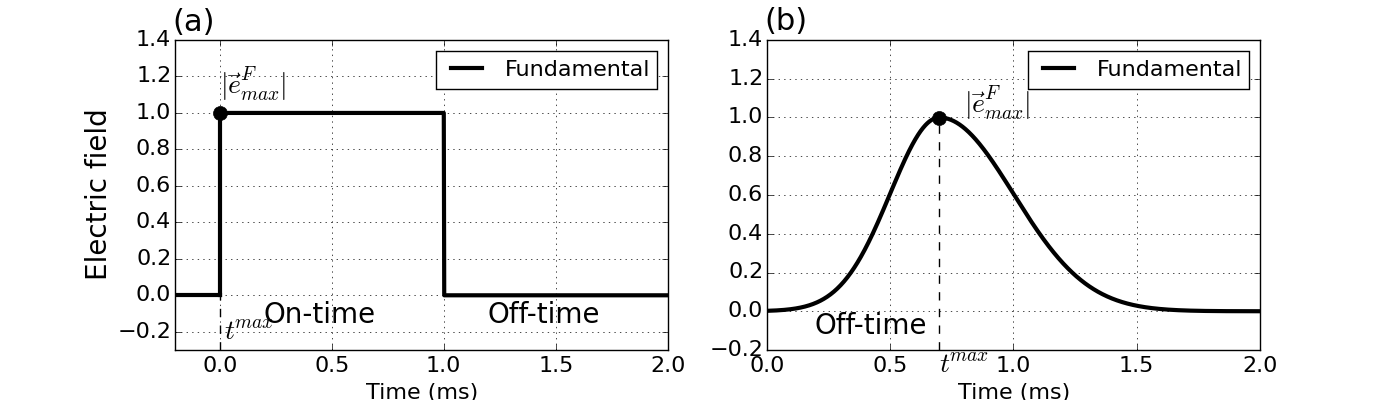
\includegraphics[width=1.0\textwidth]{figures/DCEM_F_current.png}
  \caption{Conceptual diagram for the amplitude of the fundamental electric fields. (a) EIP and (b) ISIP cases.}
  \label{F:DCEM_F_current}
\end{figure}  

%% ============================================================
%% Section. Linearization
%% ============================================================
\section{Linearization}
Following from the methodologies in EIP, our goal is to express the IP response ($\dip$) as a function of the pseudo-chargeability $(\peta(t))$ in time  $\dip(t) = J[\peta(t)]$, where $J[\cdot]$ is a linear operator which is independent of time. In doing this we first consider a general EM system which is applicable to galvanic or inductive sources. 
For any pixel  volume in the earth the amplitude and direction of the  electric field can vary dramatically  in time and this results in a complex IP charging process. If substantial polarization currents are developed however, they will correspond to a maximum electric field or reference current aligned in a constant direction. Our formulation focuses on this aspect. We assume that the final large scale IP response observed in the data is the result of  pixels being charged with an electric field in a specific direction but with a variable amplitude. Let $\e(t)$ be approximated as
\begin{equation}
  \e(t) \approx \eref w^e(t),
  \label{eq: e_with_eref}
\end{equation}
where $w^e(t)$ is defined as:
\begin{equation}
  w^e(t) = \left\{ 
  \begin{array}{l l}
    w^{ref}(t) & w^{ref}(t) \ge 0 \\
    0 & \text{if } w^{ref}(t) < 0, 
  \end{array}\right.
  \label{eq: we}
\end{equation}
with
\begin{equation}
  w^{ref}(t) = \frac{\e^F(t)\cdot\eref}{\eref\cdot\eref}.
  \label{eq: wref}
\end{equation}
Here $w^{ref}(t)$ is a dimensionless function that prescribes the time history of the electric field at each location along the direction of the chosen reference electric field ($\eref$).  Negative values of  $w^{ref}(t)$ are set to zero in accordance with our conceptual model that polarization currents have an opposite direction to the reference current (equation (\ref{eq:polarization_current_concept})).

Polarization current, $\j^{pol}$ can be approximated with equation (\ref{eq: intrinsic_peta}) as
\begin{eqnarray}
  \j^{pol}(t) \approx - \peta^{I}(t)\otimes w^e(t)\jref,
\end{eqnarray}
and substituting this into equation (\ref{eq:IP_current}) yields
\begin{eqnarray}
  \j^{IP}(t) \approx \siginf\e^{IP}(t) - \peta^{I}(t)\otimes w^e(t)\jref.
\end{eqnarray}
We redefine the pseudo-chargeability as
\begin{equation}
    \peta(t) = \peta^{I}(t)\otimes w^e(t),
    \label{eq: pseudochargeability}
\end{equation}
and this yields
\begin{eqnarray}
  \j^{IP}(t) \approx \siginf\e^{IP}(t) -\jref\peta(t).
  \label{eq: jip_EMIP}
\end{eqnarray}

The first term, $\siginf e^{IP}(t)$ is usually omitted (\cite{Smith1988a}). Here we include it and explore the conditions in which it is important. 
Because the reference current is static, any time-dependency in the polarization currents is encapsulated in the pseudo-chargeability. The buildup and decrease of polarization currents is a slow process and we assume therefore that this process does not produce induction effects ($\frac{\partial \b^{IP}}{\partial t} \approx 0$) and therefore we can write 
\begin{equation}
  \e^{IP} \approx  \e^{IP}_{approx} = -\grad\phi^{IP}.
  \label{eq: eip_approx}
\end{equation}
%% redundant but comment on what we ignored  
% Using Helmholtz decomposition, $\e$ can be decomposed as 
% \begin{equation}
%   \e^{IP}=-\vec{a}^{IP}-\grad\phi^{IP},
%   \label{eq: eip_helmholtz}
% \end{equation}
% where $\vec{a}$ and $\phi$ is electric vector and scalar potentials, respectively and $\div\vec{a}=0$. 
% Physically, $\vec{a}$ and $\phi$ indicate charge buildup and EM induction effects, which induce galvanic and vortex currents, respectively.
% Based on this decomposition, we make another assumption:
% \begin{equation}
%   \e^{IP} \approx  \e^{IP}_{approx} = -\grad\phi^{IP},
%   \label{eq: eip_approx}
% \end{equation}
% which means $\e^{IP}$ term in equation (\ref{eq: jip_EMIP}) is dominated by galvanic effect ($\vec{a}^{IP} \approx 0$). 

By taking the divergence of  equation (\ref{eq: jip_EMIP}), substituting  $\e^{IP}$ with equation (\ref{eq: eip_approx}), and carrying out some linear algebra, we obtain
\begin{equation}
  \phi^{IP}(t) \approx -[\div \siginf\grad]^{-1}\div\jref\peta(t).
  \label{eq: phiIPapprox_general}
\end{equation}
By applying the gradient we obtain 
\begin{equation}
    \e^{IP}_{approx} = \grad[\div \siginf\grad]^{-1}\div\jref\peta(t).
    \label{eq: eip_approx_full}
\end{equation}
Thus, the electric field due to the IP effect can be expressed as a function of $\peta(t)$ in time. 
This form is also applicable to the  EIP case.   

For an inductive source, the data is often either $\b$ or its time derivative and hence we also need to compute $\b^{IP}$ or its time derivative.
For this, we first compute $\j^{IP}$ then use Biot-Savart law to compute $\b^{IP}$ or $\frac{\partial \b^{IP}}{\partial t}$. 
Substituting equation (\ref{eq: eip_approx_full}) into equation (\ref{eq: jip_EMIP}), approximated IP current density, $\j^{IP}_{approx}$ can be expressed as
\begin{equation}
  \j^{IP}(t) \approx \j^{IP}_{approx} = \bar{S}\jref\peta(t),
  \label{eq: jip_approx}
\end{equation}
where
\begin{equation}
  \bar{S} = \siginf\grad[\div \siginf\grad]^{-1}\div-\bar{I}
\end{equation}
and $\bar{I}$ is an identity tensor. 
Applying Biot-Savart law we have:
\begin{equation}
  \b^{IP}_{approx}(\vec{r}; t) = \frac{\mu_0}{4\pi}\int_{\Omega}  \frac{\bar{S}\j^{\ ref}(\vec{r}_s)\times\hat{r}}{|\vec{r}-\vec{r}_s|^2}\peta(t)d\vec{r}_s.
  \label{eq: BiotbIP_approx}
\end{equation}
Omitting $\siginf\e^{IP}$ in $\j^{IP}$ simplifies the tensor, $\bar{S}$ as $-\bar{I}$. 
In this situation, the IP current is same as the polarization current, and always has opposite direction to the reference current. 
This reversed current with Biot-Savart law provides physical understanding of the negative transients in ATEM data when the earth include a chargeable body. 

Oberved data often time derivative of $\b$, hence by taking time derivative to the equation (\ref{eq: BiotbIP_approx}), we obtain
\begin{equation}
  -\frac{\partial\b^{IP}_{approx}}{\partial t}(\vec{r}; t) = \frac{\mu_0}{4\pi} \int_{\Omega}  \frac{\bar{S}\eref(\vec{r}_s)\times\hat{r}}{|\vec{r}-\vec{r}_s|^2} \Big( -\frac{\partial \peta(t)}{\partial t} \Big) d\vec{r}_s.
  \label{eq: BiotbIPdt_approx}
\end{equation}
Here we have chosen to keep the minus signs in equation (\ref{eq: BiotbIPdt_approx}) so that the sign of input of the kernel, $-\frac{\partial \peta(t)}{\partial t}$ is positive when $\peta(t)$ is decaying in time. 
Accordingly, the IP datum is determined to $-\frac{\partial\b^{IP}}{\partial t}$. 

The IP fields shown in equations (\ref{eq: eip_approx_full}), (\ref{eq: BiotbIP_approx}) and (\ref{eq: BiotbIPdt_approx}) are linear functionals of $\peta(t)$ and that $\peta(t)$ incorporates all of the time dependencies. The linear relationship can be discretized in space as
\begin{equation}
  \mathbf{d}^{IP}_i = \mathbf{J}\peta_i,
  \label{eq: dIP_lineareq}
\end{equation}
where $\mathbf{J}$ is corresponding sensitivity matrix and the subscript $i$ indicates $i^{th}$ time channel. 
In particular when the observed data is time derivative of $\b$, the linear relationship can be written as 
\begin{equation}
  \mathbf{d}^{IP}_i = \mathbf{J}(-\frac{\partial \peta}{\partial t}\Big|_i).
  \label{eq: dIP_lineareq_dbdt}
\end{equation}
A detailed description for the discretization of the linearized kernel is shown in sections \ref{section:maxwell_discrete} and \ref{section:linearkernel_discrete}. 
The representation in equation (\ref{eq: dIP_lineareq}) is valid for galvanic and inductive sources but the two assumptions: : a) $\e \approx \eref w^e(t)$ and b) $\e^{IP} \approx -\grad\phi^{IP}$ need to be tested numerically for the case of inductive sources. 

%% =============================================================================
%% Section. IP inversion methodology
%% =============================================================================

\section{IP inversion methodology}

%%% ===========================================================================
%%% SUBSECTION
\subsection{3D IP inversion with a linearized kernel}
The linear inverse problem to recover chargeability is straightforward and is described in \cite{doug1994}. 
We rewrite equation (\ref{eq: dIP_lineareq}) as
\begin{eqnarray}
  \mathbf{d}^{pred} = \mathbf{J}\mathbf{m},
  \label{eq9}
\end{eqnarray}
where $\mathbf{J}$ is the  sensitivity matrix of linear problem, which corresponds to $\mathbf{J}$ shown in equation (\ref{eq: dIP_lineareq}) 
Here, $\mathbf{d}^{pred}$ is IP responses at $i^{th}$ time channel ($\mathbf{d}^{IP}_i$), $\mathbf{m}$ is distributed model parameters, which can be either $\peta_{i}$ or $-\frac{\partial \peta}{\partial t}\big|_i$. 
In our work here we invert each time channel of $d^{IP}$, separately. 

The solution to the inverse problem is the model $\mathbf{m}$ that solves the optimization problem
\begin{eqnarray}
  minimize \ \phi =  \phi_d(\mathbf{m}) + \beta\phi_m(\mathbf{m})\nonumber \\
  s.t. \ 0 \le \mathbf{m},
  \label{eq10}
\end{eqnarray}
where $\phi_d$ is a measure of data misfit, $\phi_m$ is a user defined model objective function and $\beta$ is regularization or trade-off parameter. We solve this optimization problem using projected Gauss-Newton method (\cite{Kelley}). 
The value of $\beta$ in the iteration of this non-linear inversion determined using cooling technique where the $\beta$ is progressively reduced from some high value and the inversion stopped when the tolerance is reached (cf. \cite{Kang2014}). 

We use the sum of the squares to measure data misfit
\begin{eqnarray}
  \phi_d = \| \mathbf{W_d}(\mathbf{A}\mathbf{m}-d^{obs}|)\|^2_2 =
  \sum^N_{j=1}(\frac{\mathbf{d}^{pred}_j-\mathbf{d}^{obs}_j}{\epsilon_j}),
  \label{eq11}
\end{eqnarray}
where $N$ is the number of the observed data and $\mathbf{W_d}$ is a diagonal data weighting matrix which contains the reciprocal of the esitmated uncertainty of each datum ($\epsilon_j$) on the main diagonal,  $\mathbf{d}^{obs}$ is a vector containing the observed data, $\mathbf{d}^{pred}$ is a vector containing calculated data from a linear equation given in equation (\ref{eq9}).
The model objective function, $\phi_m$ is a measure of amount structure in the model and upon minimization this will generate a smooth model which is close to a reference model, $m_{ref}$. 
We define $\phi_m$ as
\begin{eqnarray}
  \phi_m = \| \alpha_s\mathbf{W}_s\mathbf{W}(\mathbf{m}-\mathbf{m}_{ref})\|^2_2+
       \| \alpha_x\mathbf{W}_x\mathbf{W}(\mathbf{m}-\mathbf{m}_{ref})\|^2_2+ \nonumber \\
       \| \alpha_y\mathbf{W}_y\mathbf{W}(\mathbf{m}-\mathbf{m}_{ref})\|^2_2+
       \| \alpha_z\mathbf{W}_z\mathbf{W}(\mathbf{m}-\mathbf{m}_{ref})\|^2_2,
  \label{eq12}
\end{eqnarray}
where $\mathbf{W}_s$ is a diagonal matrix, and $\mathbf{W}_x$, $\mathbf{W}_y$ and $\mathbf{W}_z$ are discrete approximations of the first derivative operator in $x$, $y$ and $z$ directions, respectively.  
The $\alpha$'s are weighting parameters that balance the relative importance of producing small or smooth models.

We are inverting each time channel of $\dip$ datum, separately. Thus, we may not have intrinsic depth resolution in most cases, unless the TEM survey include geometric sounding information. This can be obtained by multiple receivers for each transmitter, which have different offsets. To compensate for this, and similar to the magnetic inversion (\cite{LiMag3D}), we apply depth weighting through model weighting matrix ($\mathbf{W}$):
\begin{equation}
    \mathbf{W} = \mathbf{diag}(\mathbf{z-z_0})^{1.5},
    \label{eq: weight_mat}
\end{equation}
where $\mathbf{z}$ and $\mathbf{z_0}$ are discretized depth locations and reference depth in 3D domain.

%% ===========================================================================
%% SUBSECTION
\subsection{Extracting intrinsic IP parameters}
\label{section: extract_intrinsicIP}
The output of our IP inversion is 3D distribution of the pseudo-chargeability at multiple time channels. 
As its name suggests, pseudo-chargeability is not an intrinsic IP parameter like chargeability, but it is convoluted property between $\peta^{I}(t)$ and $w^{e}(t)$:
\begin{equation}
  \peta(t) = \peta^{I}(t)u(t) \otimes w^e(t),
  \label{eq: pseudochargeability_petaI}
\end{equation}
with the definition of intrinsic pseudo-chargeability (equation (\ref{eq: intrinsic_peta})).
Assuming a Debye model ($c$=1), we obtain
\begin{equation}
    \peta^{I}(t) = \frac{\eta}{(1-\eta)\tau}e^{-\frac{t}{(1-\eta)\tau}},
    \label{eq: intrinsic_peta_debye}
\end{equation}
Since we have $\siginf$ we can compute $w^e(t)$, which is time history of the electric field. 
Accordingly, we can unravel the recovered pseudo-chargeability to extract intrinsic IP parameters such as chargeability($\eta$) and time constant ($\tau$). 
We use a gradient-based optimization, we need the sensitivity function for the pseudo-chargeability (equation (\ref{eq: pseudochargeability_petaI})) with regard to $\eta$ and $\tau$. 
To simplify this procedure, we rewrite intrinsic pseudo-chargeability as 
\begin{equation}
  \peta^{I}(t) = a e^{-bt},
\end{equation}
where $a = \frac{\eta}{(1-\eta)\tau}$ and $b = \frac{t}{(1-\eta)\tau}$. 
Then we take derivative of $\peta(t)$ with regard to $a$ and $b$:
\begin{equation}
  \frac{\partial \peta(t)}{\partial a} = e^{-bt} \otimes w^e(t),
\end{equation}
\begin{equation}
  \frac{\partial \peta(t)}{\partial b} = -ate^{-bt} \otimes w^e(t).
\end{equation}
With these sensitivity functions, we can set up an inverse problem, and recover $a$ and $b$. 
Chargeability and time constant can be obtained by using $a$ and $b$:
\begin{equation}
  \eta =  \frac{1}{(1-a/b)b},
\end{equation}
\begin{equation}
  \tau =  \frac{a}{b}.
\end{equation}
We apply this inversion separately to each cell in the recovered pseudo-chargeability  in a manner similar to Yuval and Oldenburg.
For the better representation of time-dependent conductivity, a different parameterization such as stretched-exponential (CITEStretchedExp) or Cole-Cole with variable $c$ can be implnmented. 

%%% ===========================================================================
%%% SUBSECTION
\subsection{Handling multiple transmitters in ATEM surveys}
\label{subsection: Handling multiple transmitters in ATEM surveys}
The work for inductive sources in the previous sections has been developed for a single transmitter and  3D information about chargeability can be obtained if there are multiple receivers. For ATEM data however, we have only a single receiver location for each transmitter but we have multiple transmitter locations. 
Our goal is to alter the problem to work with an effective pseudo-chargeability. 

% This includes all grounded surveys with multiple transmitters and to a single source inductive EIP surveys.
% Doug: The sensitivity depends mostly on geometry but also upon the fundamental currents for each transmitter. Thus both J and \tilde eta are different for each transmitter. How do we proceed with more mathematical rigor?

Considering this situation where the survey includes multiple transmitters, we define IP datum for $k$-th transmitter as 
\begin{equation}
  \dip_k(t) = J_k[\peta_k (t)], \ \ k=1, \ldots, nTx,
  \label{eq: dip_kthTx}
\end{equation}
where $nTx$ is the number of transmitters. Effective pseudo-chargeability, $\peta_{eff}$ can be easily determined for an idealistic situation when pseudo-charegeability for all transmitters are same. Then we can rewrite equation (\ref{eq: dip_kthTx}) as 
\begin{equation}
  \dip(t) = J[\peta_{eff}(t)].
  \label{eq: dip_eff}
\end{equation}
Here $\dip$ and $J[\cdot]$ include all data from every tranmitter-receiver pair. From the definition of the pseudo-chargeability, we regonize that the above condition can be satisfied when $w^e_k(t)$ for every transmitter is same. 
Any time variation in fundamental electric field for the EIP case is same as applied current waveform as shown in Figure ~\ref{F:DCEM_F_current}a. 
As such, $w^e_k(t)$ for every transmitter is same, which makes every $\peta_k(t)$ same. 

Conversely for the ISIP case such as ATEM, this condition will not be satisfied, because time-varying feature of $w^e_k(t)$ is different for each transmitter. 
For instance, the reference time at a single pixel shown in Figure ~\ref{F:DCEM_F_current}b will be different at different transmitter locations. 
We consider this problem for the ATEM data. 
Sensitivty of the IP datum to a chargeable body will be proportional to $\sim1/r^3$ where $r$ stands for the distance between the body and transmitter location if we only treat coincident-loop system. 
Thus, IP datum far away from the body will have minor amplitude compared to one close to the body. 
Reflecting this feature, we define averaged pseudo-chargeability, $\peta_{avg}(t)$ as 
\begin{equation}
  \peta_{avg}(t) = \sum_{k=1}^{nTx} a_k \peta_k(t),
  \label{eq: pseudo-chargeability_avg}
\end{equation}
where a normalized weighting coefficient, $a_k$ is defined as 
\begin{equation}
  a_k = \frac{\| \mathbf{J}^{blk}_k \|_2  }{\sum_{k=1}^{nTx} \| \mathbf{J}^{blk}_k \|_2 }.
\end{equation}
Here $\mathbf{J}^{blk}_k$ indicates Jacobian matrix corresponding to some cells in a chargeable body at $k$-th transmitter. 
This normalized weighting coefficient wll include not only geometric decaying feature of IP response from the body, but also effect of anomalous conductivity structure on IP response. 
Therefore, the averaged pseudo-chargeability using this normalized weighting will effectively incorporate physics behind. 

By using geophysical inversion with IP functional shown in equation (\ref{eq: dip_eff}), we recover effective pseudo-chargeability which explains the observed IP data. 
The reliability of this effective pseudo-chargeability will be suported by evaluating $\dip$ data computed by using equation (\ref{eq: dip_eff}) with the averaged pseudo-chargeabiliy, and comparing those with true $\dip$ data. 
% Doug
% This includes all grounded surveys with multiple transmitters and to a single source inductive EIP surveys.


%%% ===========================================================================
%%% SUBSECTION
\subsection{IP inversion procedure}
As seen in the previous sections the extraction of IP information from TEM data has multiple steps. These include: (1) invert TEM data and recover a 3D conductivity model ($\sigma_{est}$). 
(2) Forward modelling $\sigma_{est}$ to obtain the fundamental response $d^F$ and subtracting it from the observations to obtain $\dip$ data.
(3) Invert  $\dip$ data to recover pseudo-chargeability model at individual time channels using the relationship in equation (\ref{eq: dIP_lineareq}). 
(4) Further process the inversion outputs at multiple time-channels  to estimate the Cole-Cole, or equivalent IP parameters.

In the following we investigate each of the above steps via numerical simulations and test the validity of our assumptions. 

%% =============================================================================
%% Section. Numerical experiments
%% =============================================================================

\section{Numerical experiments}
\label{section: numerical_examples}
For our numerical experiments we concentrate upon coincident loop ATEM surveys. This choice is made because of the observed negative transients that are direct indicators of IP phenomena (\cite{Kratzer2012,Kang2015a,Kang2015b,Doug2015}), and the extensive  use of this survey  by industry.  

We begin with a simple IP model composed of  a chargeable block in a half-space as shown in Figure~\ref{F: IPModel}.
Cole-Cole parameters of block are  $\eta=$0.2, $\tau=$0.005 and $c=$1.
The conductivity  of the half-space, ($\sigma_1$) is  $10^{-3}$ S/m, whereas $\sigma_2$, 
the conductivity at infinite frequency ($\siginf$) for the chargeable body, is variable.  
We consider three cases: a) canonical ($\sigma_2=\sigma_1$), b) conductive ($\sigma_2=10^2\times\sigma_1$) and c) resistive models ($\sigma_2=10^{-2}\times\sigma_1$).
The 3D earth is discretized with  $50\times50\times50$ m core cells and the number of cells in the domain is $41\times41\times40$.
The size of the chargeable body is $250\times250\times200$ m and the top boundary is located  $50$ m below the surface.
EMTDIP code (\cite{Marchant2014}) is used to compute forward ATEM responses that include IP effects. The survey consisting of 11 soundings along each of 11 lines is shown in Figure \ref{F: IPModel}a.
Data are from a  coincident-loop system and both Tx and Rx located 30 m above the surface; the radius of the loop is 10 m.
A step-off transmitter waveform is used and the range of the observed time channel is 0.01-60 ms. The observed responses can be either vertical component of $\b$ or $\frac{\partial \b}{\partial t}$.

% Seogi
% Needs some correction later
In this section, we first decompose the observed responses and the total currents into fundamental and IP portions to aid in the basic understanding of IP effects in ATEM data. 
Second, we validate the linearized kernel by computing the approximate IP current and IP responses, and comparing these  with the true values. 
Third, we investigate the feasibility of an equivalent pseudo-chargeability in 3D IP inversion. 
Fourth, we invert the IP data and recover 3D distributions of pseudo-chargeability at multiple times.  Lastly, we use the recovered pseudo-chargeabilities to examine the potential to extract intrinsic Cole-Cole parameters. 

\begin{figure}[htb]
  \centering
  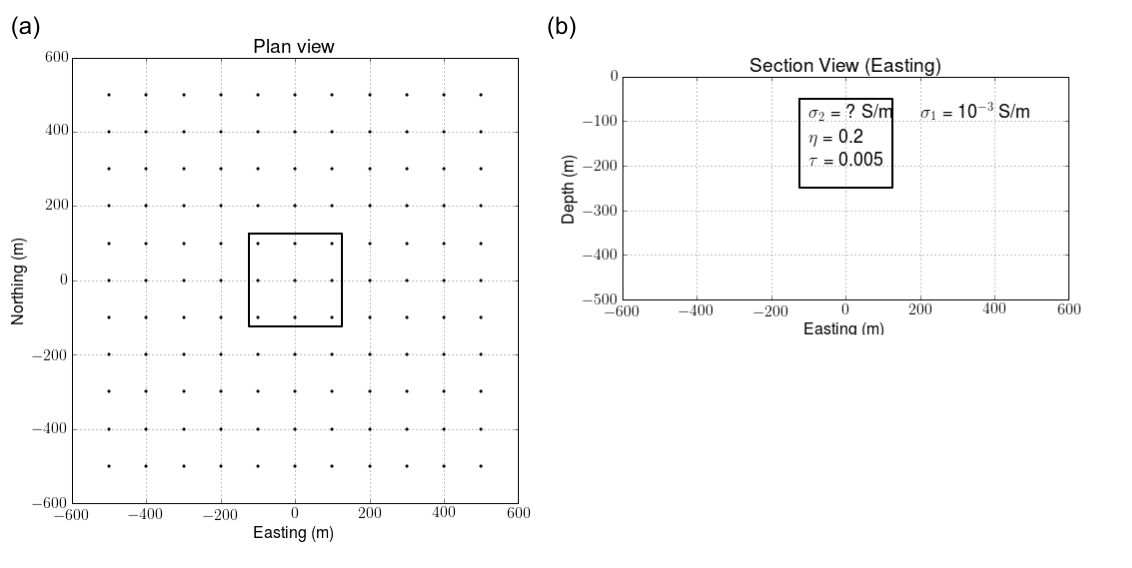
\includegraphics[width=1.0\textwidth]{figures/IPModel.png}
  \caption{Plan (a) and section b) views of the IP model. Dashed line in (a) contours the boundary of the IP body. Solid circles in (a) denotes the sounding locations.}
  \label{F: IPModel}
\end{figure}
\clearpage

%%% ===========================================================================
%%% SUBSECTION
\subsection{IP responses}
Using EMTDIP code and carrying out two simulations, we compute the IP data via subtraction in equation (\ref{eq: IPdatum_syn}).
Figure \ref{F:Three_IPresp} shows the observed, fundamental, and IP responses at a sounding location above the center of the chargeable body for (a) canonical, (b) conductive and (c) resistive models. Both $b_z$ and $-\frac{\partial b_z}{\partial t}$ data are shown. 
The IP effects are most noticeable for the conductive body and we turn attention to this example first. The IP response starts to significantly affect the observations near 0.6 ms and the observed responses show a sign reversal near 1 ms. Beyond that time the signal is completely dominated by the IP. The dashed line in Figure \ref{F:Three_IPresp}c shows that after turn-off of the transmitter current,  the IP current increases (as inferred by the magnitude of the $b_z$ field) until about 1 ms and then decreases. We interpret this in terms of charging and discharging phases and a vertical dashed line in the figure defines the two phases. In the charging phase at early times the EM effects dominate and IP signals are not expected to be observed. In the discharging phase, which occurs at  later time, the IP effects may eventually dominate the EM effects. The maximum of the $b_z^{IP}$ corresponds to the zero crossing for $\frac{\partial b_z^{IP}}{\partial t}$ but the times at which the IP signal becomes dominant are delayed compared to $b_z^{IP}$. By comparing the observations with the fundamental fields we see that the IP signal could be recognized in the $b_z$ data near 0.7 ms and near 2.0 ms in the $\frac{\partial b_z}{\partial t}$ data.

The plots for the canonical and resistive bodies show that the time that separates charging and discharging occurs earlier than for the conductive body. This is a reflection that the fundamental currents take a long time to decay in a conductor. For the canonical body, significant difference between the measured responses and the fundamental fields occur about 0.9 ms for $b_z$ and about 2 ms for $\frac{\partial b_z}{\partial t}$. The amplitudes of the IP responses are significantly smaller than those for the conductor.  Lastly, there is little IP signal for the resistive body; the IP signal much smaller than the fundmental response in given time range. After 50 ms the IP signal is significantly decayed, and hence the observed response is almost identical to fundamental one for all three cases. 

The decay curves from a sounding location  provides insight about the IP response but more is gleaned by looking at data from all  sounding locations in the ATEM survey. We focus on $b_z^{IP}$ for the conductive block at selected time channels. Figure \ref{F:IPresp_Plan} shows interpolated maps of the observed, fundamental and IP responses at (a) 0.86 ms and (b) 6.7 ms which are respectively included in the charging and discharging times. 
At 0.86 ms, the observations are dominated by the fundamental response and no negative values,  which are the signature of the IP effect, are observed. Subtracting the fundamental however, yields a residual $\dip$ data map that has a strong negative. This  example  shows that our EM decoupling procedure has worked satisfactorily.  At 6.7 ms, obtaining good IP data is easier because the observed data already show negative values. There is still a weak fundamental field and the subtraction process improves the $\dip$ response. The $\dip$ data at  0.86 ms and 6.7 ms shown in Figure \ref{F:IPresp_Plan} are of sufficient quality to be inverted. The decoupling has been carried out using the known background conductivity $\siginf$ which, in reality must be estimated. We address this issue later. 

\begin{figure}[htb]
  \centering
  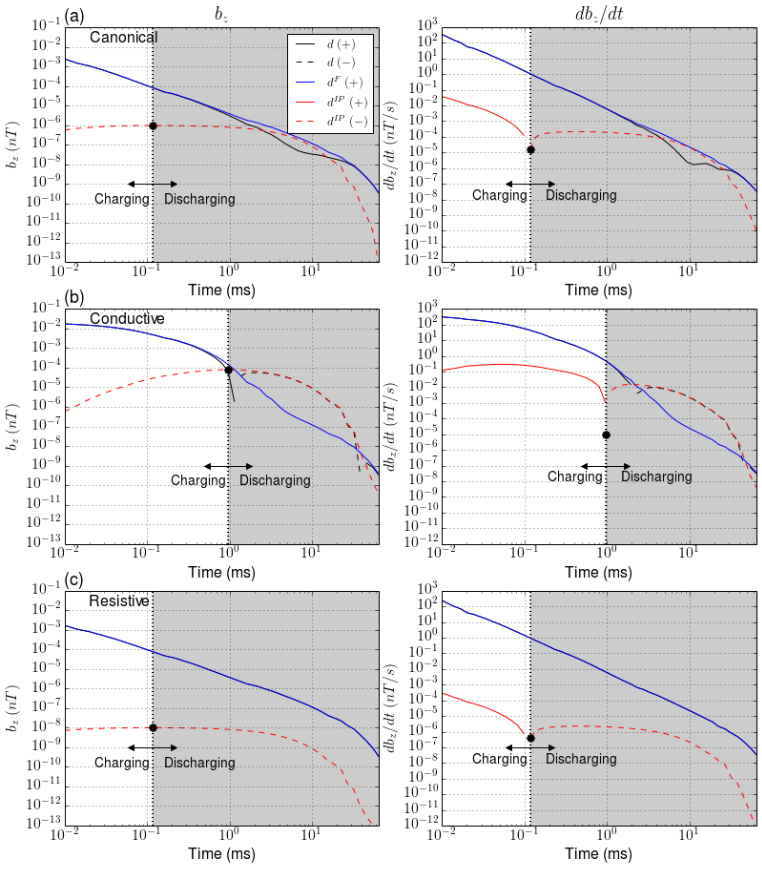
\includegraphics[width=1.\textwidth]{figures/Three_IPresp.png}
  \caption{Time decaying curves of observation ($d$; black line), fundamental ($d^F$; blue line) and IP ($\dip$; red line) responses. All three cases: (a) canonical, (b) conductive and (c) resistive are presented. Right and left panels show $b_z$ and $\frac{\partial b_z}{\partial t}$. Black dotted line indicates the maximum polarization time.}
  \label{F:Three_IPresp}
\end{figure}
\begin{figure}[htb]
  \centering
  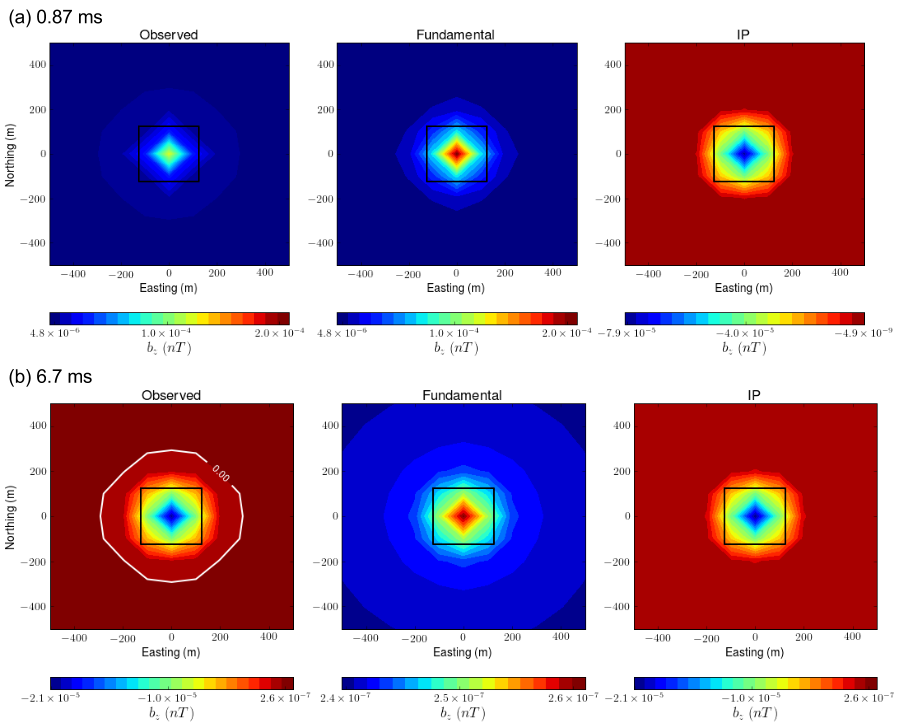
\includegraphics[width=1.\textwidth]{figures/IPresp_Plan.png}
  \caption{Interpolated maps of observed (left panel), fundamental (middle panel) and IP (right panel) responses. Two time channels at (a) 0.86 ms and (b) 6.7 ms are presented. White line contours zero-crossing in the observed response.  
  }
  \label{F:IPresp_Plan}
\end{figure}
\clearpage

%%% ===========================================================================
%%% SUBSECTION
\subsection{Polarization currents}
%Need some intro. 
To derive the linearized kernel for the IP responses, we made two main assumptions: a) $\e \approx \eref w^e(t)$ and b) $\e^{IP} \approx -\grad\phi^{IP}$. We numerically test these assumptions and analze physics behind.

The first assumption may not be reasonable when the earth include either a conductor or a resistor because the direction of electric field dynamically changes in time due to the induced current. 
However, we only apply this assumption for the polarization current, and the rationale behind this was that polarization currents developed from charging or discharging process will correspond to a reference current alinged in constant direction. 
Since $\dsig(t)$ has non-zero values only in a chargeable body, so the polarization current does based on equation (\ref{eq:polarization_current}). 
Choice of the maximum electric field as the reference electric field includes the time history of the fundamental electric field (equation (\ref{eq:reference_electricfield})). 
Similarly, the reference current includes the time history of  fudamental current. 
We first analyze this reference current shown in Figure ~\ref{F:ReferenceCurrent}. 
Here a transmitter is located at (-200 m, 0 m, 30 m) and marked as white solid circle, where ($\cdot, \cdot, \cdot$) means a point at (easting, northing, depth).  
The fundamental current for canonical model is circular, centered to the transmitter location, and is decaying as further away from this location. This feature is clearly captured in the referecne current as shown in Figure ~\ref{F:ReferenceCurrent}a. 
In the chargeable body, most of the currents is alinged in northing direction. 
Different from canonical case, when the earth contain a conductor, vortex current will be induced from the conductor, whereas the similar circular current centered to transmitter location still exists.  
Figure ~\ref{F:ReferenceCurrent}b shows that the reference current, which effectively incorporate both induced currents from the half-space earth and the embedded conductor.  
Especially in the body, the reference current is composed of linear currents alinged in northing direction and rotating currents in clockwise and counter-clockwise at plan and section view maps, respectively. 

To test our assumption, we present polarizatin currents computed using equaiton (\ref{eq:polarization_current}). 
Figures ~\ref{F:Polarizationcurrent_early} and ~\ref{F:Polarizationcurrent_late} show the plan and section view maps of the polarization currents at 0.86 ms and 6.7 ms, respectively. 
For canonical model, polarization current show linear current alingned in northing direction, but opposite direction to the reference current. 
Similar to the amplitude of the reference current, closer volumes to transmitter location in the body has greater amplitude of the polarization current. 
Direction of polarization currents for conductive case is also aligned with the opposite direction of the reference current.
Comparing two different times of the polarization currents show that direction of the polarizaiton currents almost constant at these times, whereas their amplitudes decrease as time increases. 
These times might be included in discharging phase, and this approximation is reasonable. 
At much earlier times in charging phase, performance of the approximation might be poor. 

% Seogi: Remove Rx in the figure
\begin{figure}[htb]
  \centering
  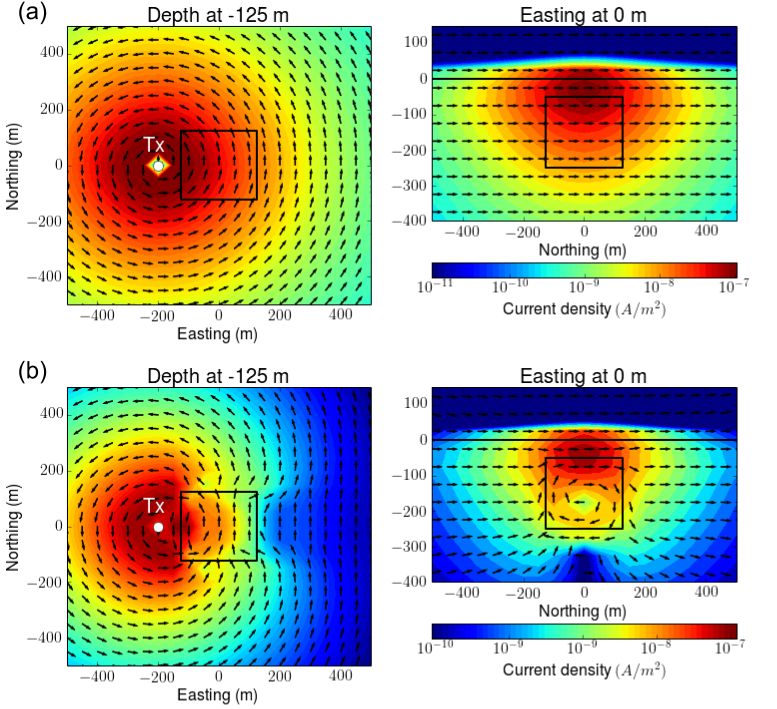
\includegraphics[width=1\textwidth]{figures/ReferenceCurrent.png}
  \caption{Maps of reference currents: (a) canonical and (b) conductive models. Left and right panel show plan and section views at -125 m-depth and 0 m-easting, respectively. A transmitter is located at (-200 m, 0 m, 30 m). Black arrows and shaded value indicate the direction and amplitude of the current, respectively. Black solid outlines boundary of the surface or the chargeable body.}
  \label{F:ReferenceCurrent}
\end{figure}

\begin{figure}[htb]
  \centering
  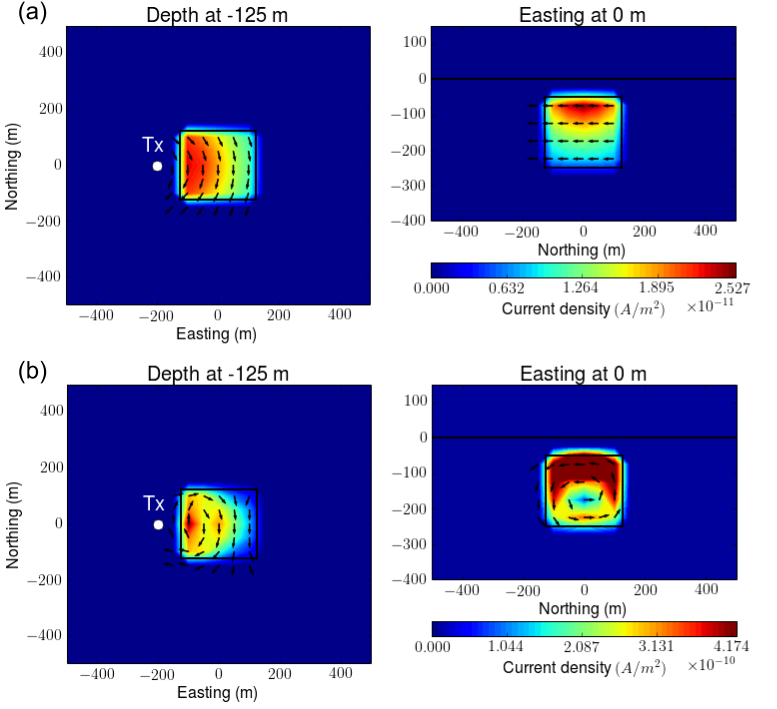
\includegraphics[width=1\textwidth]{figures/Polarizationcurrent_early.png}
  \caption{Maps of polarization currents: (a) canonical and (b) conductive models at 0.86 ms. Left and right panel show plan and section views at -125 m-depth and 0 m-easting, respectively. A transmitter is located at (-200 m, 0 m, 30 m). Black arrows and shaded value indicate the direction and amplitude of the current, respectively. Black solid outlines boundary of the surface or the chargeable body.}
  \label{F:Polarizationcurrent_early}
\end{figure}

\begin{figure}[htb]
  \centering
  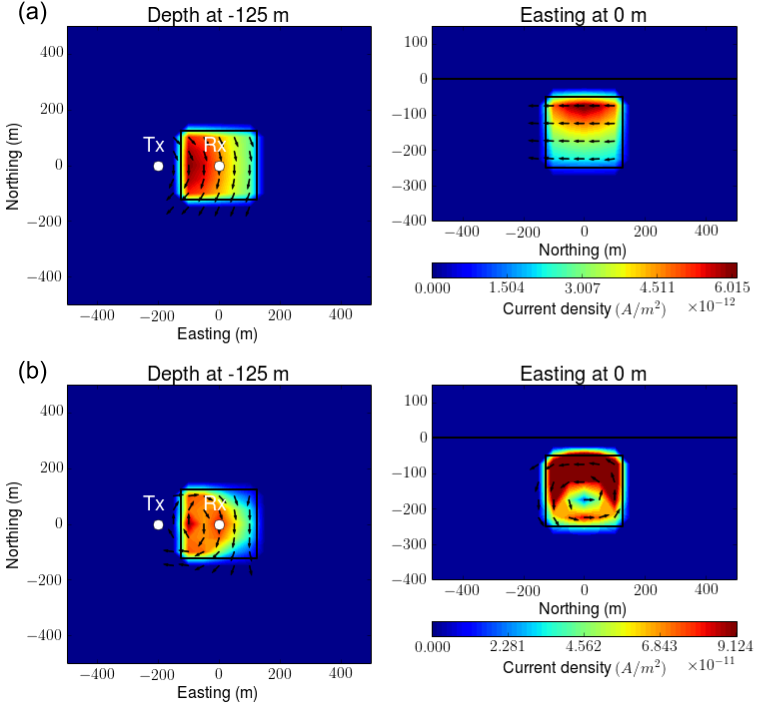
\includegraphics[width=1\textwidth]{figures/Polarizationcurrent_late.png}
  \caption{Maps of polarization currents: (a) canonical and (b) conductive models at 6.7 ms. Left and right panel show plan and section views at -125 m-depth and 0 m-easting, respectively. A transmitter is located at (-200 m, 0 m, 30 m). Black arrows and shaded value indicate the direction and amplitude of the current, respectively. Black solid outlines boundary of the surface or the chargeable body.}
  \label{F:Polarizationcurrent_late}
\end{figure}
\clearpage

\subsection{IP currents and validations of linearization}
Different from \cite{Smith1988a}, we consider $\siginf \e^{IP}$ term in the IP current. 
Relative strength of this term in the IP current to the polarization current is always significant at the outside of the body, because the polarization current is zero here. 
To evaluate $\e^{IP}$, we use polarization current as a source term as shown in equation (\ref{eq: eip_approx}) with the second assumption: $\e^{IP} \approx -\grad\phi^{IP}$. 
For conventional EIP case, we usually consider dipolar IP response originated from the linear-shaped polarization current in a chargeable body (\cite{seigel1959}). 
However, for ISIP case with conductor this can be more complex due to the effect of induced vortex current in the polarization current (Figures \ref{F:Polarizationcurrent_early}b and \ref{F:Polarizationcurrent_late}b). 

The assumption can be mathematically represented with Helmholz decomposition. 
Using this decomposition, we let $\e^{IP} = -\grad \phi^{IP} - \vec{a}^{IP}$ with $\div \vec{a}^{IP} = 0$.
As such, we ignore inductive term: $\vec{a}^{IP}$ in $\e^{IP}$ for our assumption. 
Here $\phi^{IP}$ and $\vec{a}^{IP}$ correspondingly indicate electric scalar and vector potentials, and are related to inductive and galvanic IP effect, respectively. 
We test this assumption by numerically evaluating this decomposition. 
Figure ~\ref{F:IPcurrents_helmholtz_early} respectively show plan view maps of $\j^{pol}$, $-\siginf \vec{a}^{IP}$, and $-\siginf \phi^{IP}$ for (a) canonical, (b) conductive, and (c) resistive models at 0.86 ms.
For all three cases the polarization currents have the greatest strength in the body. 
Compared to $-\siginf \phi^{IP}$, $-\siginf \vec{a}^{IP}$ show minor strength for canonical and resistive cases, whereas strength of two currents are considerable for conductive case. 
This alludes that conductive case is the most challenging situation for this assumption.
We only showed 0.87 ms, but features on three currents does change after this time.

Using two assumptions we compute approximate IP current as shown in equation (\ref{eq: jip_approx}). 
We compare this approximate IP current with true one. 
Figures ~\ref{F:IPcurrent_PlanandSec_early} show comparison of the true and approximate IP currents for conductive case at 0.86 ms. 
Approximate IP current shows good match with true one in the body about both its direction and amplitude, whereas they get more different as further away from the body (right panel of Figure ~\ref{F:IPcurrent_PlanandSec_early}).
As time increases to 6.7 ms, approximate current converges to true one as shown in Figure ~\ref{F:IPcurrent_PlanandSec_late}.  
Finally, we evaluate IP response applying Biot-Savart law to this approximate IP current as shown in equation (\ref{eq: BiotbIP_approx}). 
Figure ~\ref{F:True_vs_approx_IPresp} show comparisons of IP responses for canonical (black), conductive (blue), and resistive (red) cases computed by applying discrete Biot-Savart operator to true (solid stars) and approximate (empty circles) IP currents. 
To test the reliability of discrete Biot-Savart operation, we also compute IP response by the subtraction of the fundamental response from the observation.
After 0.01 ms, IP responses computed from true IP current with Biot-savart law almost identical to ones computed from subtraction for all three cases. 
Approximate IP response for canonical and resitive cases almost identical to true one after 0.03 ms, whereas that for conductive case coverges to true one after 0.8 ms. 
These results consistent with that the canonical and resistive cases have earlier maximum charging time ($\sim$ 0.1 ms) than conductive case ($\sim$ 1 ms).
Overall, developed linear functional of IP response for ATEM data show good performances for all three different conductivity structures in discharging phase when the polarization current decreases. 

\begin{figure}[htb]
  \centering
  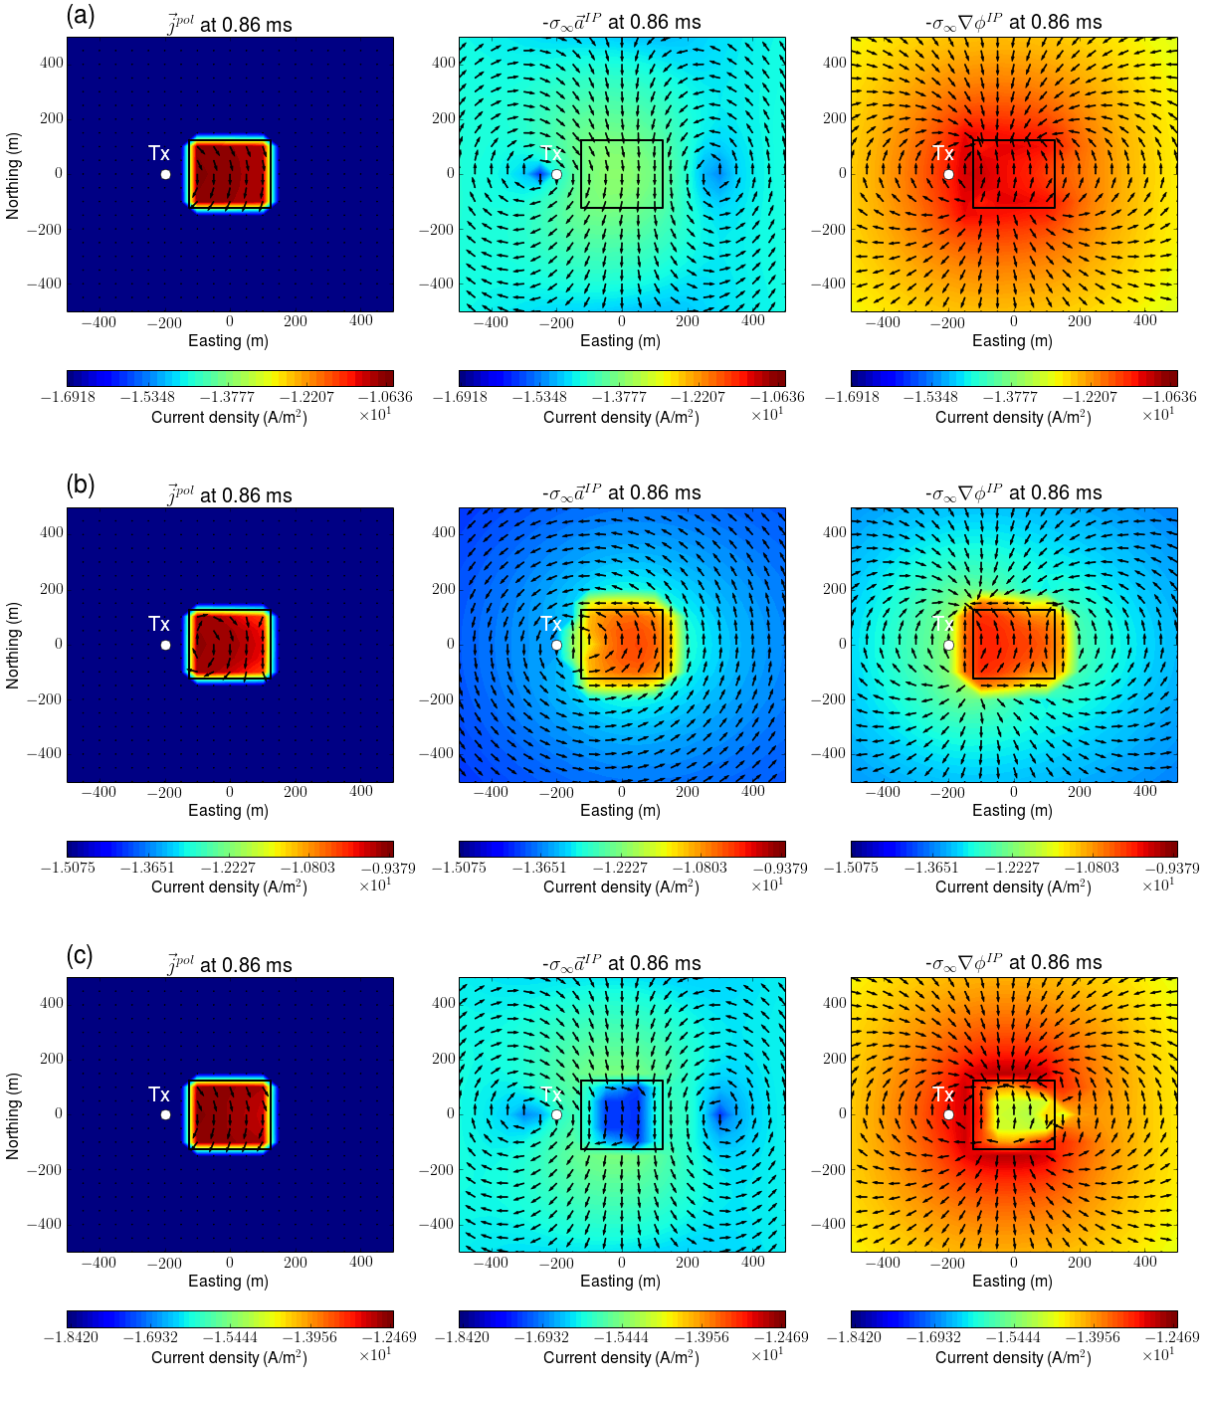
\includegraphics[width=1.\textwidth]{figures/IPcurrents_helmholtz_early.png}
  \caption{Decomposition of the IP currents as $\j^{pol}$ (left panel), $-\siginf\vec{a}^{IP}$ (middle panel), and $-\siginf\grad \phi^{IP}$ (right panel) at 0.86 ms. Plan view maps of the currents at -125 m-depth are shown. (a) Canonical, (b) Conductive, and (c) Resistive cases. }
  \label{F:IPcurrents_helmholtz_early}
\end{figure}

\begin{figure}[htb]
  \centering
  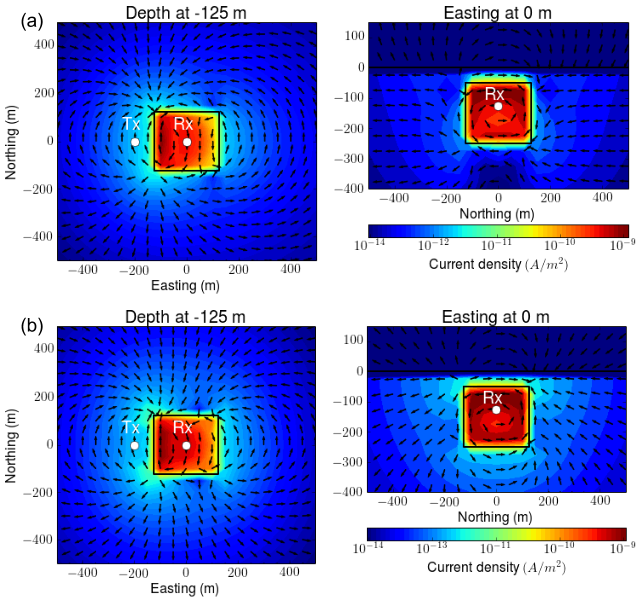
\includegraphics[width=1\textwidth]{figures/IPcurrent_PlanandSec_early.png}
  \caption{Interpolated maps of (a) true and (b) approximate IP currents at 0.86 ms. Left and right columns show plan and section view maps at -125 m-depth and 0 m-easting, respectively. }
  \label{F:IPcurrent_PlanandSec_early}
\end{figure}

\begin{figure}[htb]
  \centering
  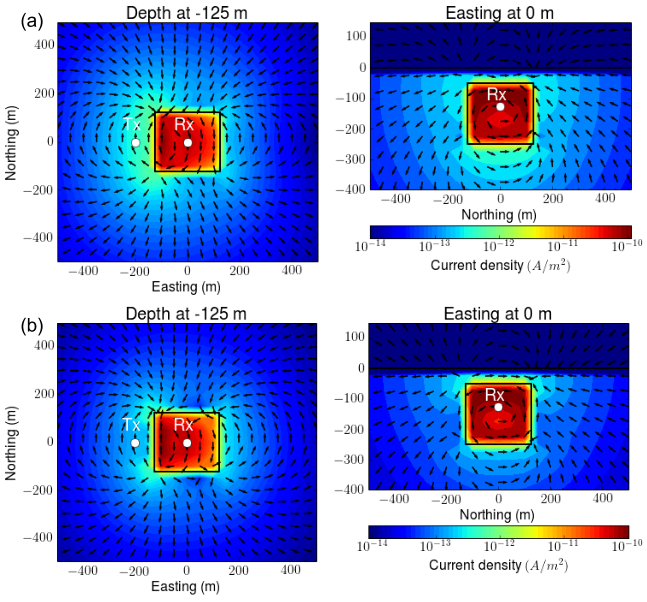
\includegraphics[width=1\textwidth]{figures/IPcurrent_PlanandSec_late.png}
  \caption{Interpolated maps of (a) true and (b) approximate IP currents at 6.7 ms. Left and right columns show plan and section view maps at -125 m-depth and 0 m-easting, respectively. }
  \label{F:IPcurrent_PlanandSec_late}
\end{figure}

\begin{figure}[htb]
  \centering
  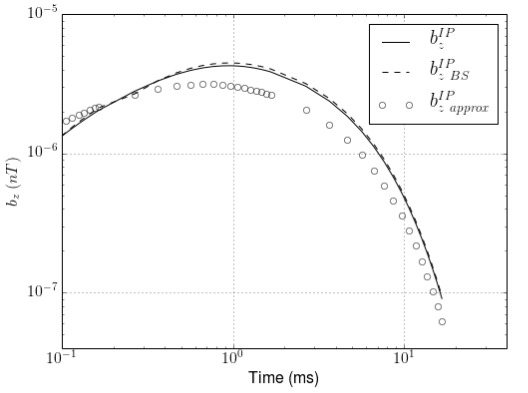
\includegraphics[width=1\textwidth]{figures/True_vs_approx_IPresp.png}
  \caption{Comparison of true and approximate IP respones ($b_z^{IP}$). Black, blue, and red color respectively indicate canonical, conductive, and resistive cases. Solid lines indicate true $b_z^{IP}$ computed by subtraction process and application of Biot-Savart to true IP current ($b_{z \ BS}^{IP}$). Empty circles presents approximate $b_z^{IP}$. }
  \label{F:True_vs_approx_IPresp}
\end{figure}
\clearpage

%%% ===========================================================================
%%% SUBSECTION
\subsection{Effective pseudo-chargeability for ATEM data}
In previous section, we showed the capability of the linear functional for a single transmitter. 
However, ATEM data include multiple transmitters yielding different pseudo-chargeability for each transmitter as we have treated in Section \ref{subsection: Handling multiple transmitters in ATEM surveys}. 
Using the effective pseudo-chargeability, we altered the problem as shown in equation (\ref{eq: dip_eff}), which later enables inverse problem recovering not pseudo-chargeability for each transmitter, but an effective pseudo-chargeability. 
Because geophysical inverse problem is non-unique, there can be multiple effective pseudo-chargeability which explains the observed IP response. 
In this section, we numerically test a feasibility of this alteration of the problem. 

For this, we rewrite equation (\ref{eq: pseudo-chargeability_avg}) as
\begin{equation}
  \peta_{avg}(t) = \peta^{I}(t)u(t) \otimes w^e_{avg}(t),
  \label{eq: pseudo-chargeability_avg_we}
\end{equation}
where 
\begin{equation}
  w^e_{avg}(t) = \sum_{k=1}^{nTx} a_k w^e_{k}(t).
  \label{eq: we_avg}
\end{equation}
Here subscript $k$ means $k$-th transmitter. 
Pseudo-chargeabilities are different for different transmitters because $w^e_k(t)$ is different. 
If they are same for every transmitter, effective chargeability can be uniquely defined, which will not be true for ATEM data. 
The averaged pseudo-chargeability includes physics behind through normalized weighting, and hence we consider this as an effective pseudo-chargeability. 
We evalute first this averaged pseudo-chargeability and then using this compute IP responses with linear functional. 
For the computation of normalized weighting, we only consider some correspoding elements of Jacobian matrix in a chargeable body ($\mathbf{J}^{blk}_k$) for each transmitter. 

We set two ways to choose some cells in a chargeable body: a) a single cell at the center of the body and (b) all cells in the body. 
For numerical experiments in this section we limit our attention to conductive case. 
Figure ~\ref{F:NormalizedWeights} show normalized weights for all transmitter locations with two choices.
For both choices, normalized weight is decaying from the center of body, whereas that for the choice of a single cell (Figure ~\ref{F:NormalizedWeights}b) show steeper decay than the other (Figure ~\ref{F:NormalizedWeights}b). 
Away from the center ($>$200m ), the normalized weights with two choices are similar. 
With these weights, we compute averaged $w^e(t)$ using equation (\ref{eq: we_avg}) for each choice. 
In Figure ~\ref{F:AveragedWe}, we present $w^e_k(t)$ (dashed lines) for every transmitter and $w^e_{avg}(t)$ (solid line with dots) at the center cell of the body. 
As expected, $w^e_k(t)$ for different transmitters are different. 
Averaged $w^e(t)$ with two different choices reach to the maximum near 1.5$\times 10^{-4}$ ms. 
After this time they are similar, whereas they have considerable difference before this time. 
Using this averaged $w^e(t)$ we first compute averaged pseudo-chargeability (equation (\ref{eq: pseudo-chargeability_avg_we})), then with this we calcuate IP responses using linear functional (equation(\ref{eq: dip_eff})). 
Figure ~\ref{F:EquivPeta_True_Approx} show the comparison of true and approximate IP responses on plan view map at 0.86 ms. 
Both approximated $\dip$ responses computed by using averaged pseudo-chargeability with the choice of a single cell (Figure ~\ref{F:EquivPeta_True_Approx}b) and all cells (Figure ~\ref{F:EquivPeta_True_Approx}c) show reasonable match with true $\dip$ response (Figure ~\ref{F:EquivPeta_True_Approx}a); the latter one slightly closer to the true ones. 
After 0.86 ms, distribution of IP response on map view does not change signficantly and both approximate $\dip$ responses show similar performances.
Same anlayses was applied to canonical and resistive cases and showed similar results, although we have not shown here. 
The results of analyses shown demonstrate that alteration of the problem to recover an effective pseudo-chargeability is reasonable. 
We will also test in following inversion examples by investigating recovered pseudo-chargeability from the inversion. 
\begin{figure}[htb]
  \centering
  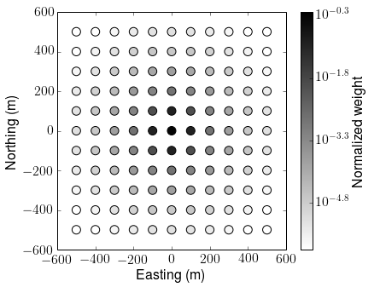
\includegraphics[width=1.\textwidth]{figures/NormalizedWeights.png}
  \caption{}
  \label{F:NormalizedWeights}
\end{figure}

\begin{figure}[htb]
  \centering
  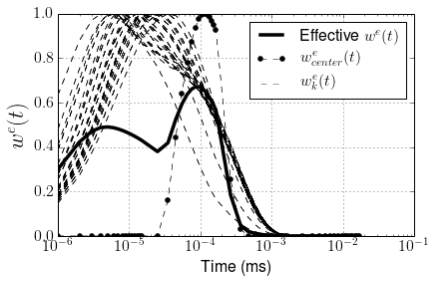
\includegraphics[width=1.\textwidth]{figures/AveragedWe.png}
  \caption{}
  \label{F:AveragedWe}
\end{figure}
\clearpage

\begin{figure}[htb]
  \centering
  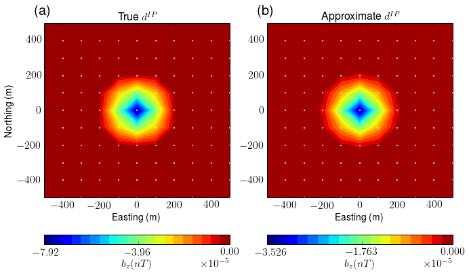
\includegraphics[width=1.\textwidth]{figures/EquivPeta_True_Approx.png}
  \caption{Comparison of (a) true and (b) approximate $b_z^{IP}$ responses at 0.86 ms on plan view map.}
  \label{F:EquivPeta_True_Approx}
\end{figure}
\clearpage


%%% ===========================================================================
%%% SUBSECTION
\subsection{3D IP inversions}
Based on the systematic validation performed in previous sections, we now proceed with 3D  inversion using our linearized sensitivityl.
We invert data at each  time channel and recover 3D pseudo-chargeability at multiple times. 
Our 3D inversion is based upon \cite{doug1994,Li2000}, and it requires some choices for inversion parameters. 
Because we invert each time channel of the IP datum, separately, the number of the data in the inversion is same as the number of soundings. 
For data uncertainties, we used one percent of the maximum amplitude of the observed data (0.1$max(|\mathbf{d}^{obs}|)$). Coefficients for smallness and smoothness are set to $\alpha_s=10^{-5}$ and $\alpha_x=\alpha_y=\alpha_z=1$, respectively. The reference model is zero and we also applied a depth weighting and positivity constraint on the pseudo-chargeablity. The need for a depth weighting arises because the sensitivity function $J$ is primarily controlled by a $1/r^3$ decay associated with the Biot-Savart kernels.  Thus an ATEM data set is not unlike commonly acquired  magnetic data where it is well established that a depth weighting is required to image objects at depth.  The following example illustrates this.  

We first generate IP responses at a single time using the linearized kernel by assuming that the pseudo-chargeability is unity inside the body and zero outside, as shown in  Figure \ref{F:Depthweight}(a). 
Figure \ref{F:Depthweight}(b) shows the recovered pseudo-chargeability without depth weighting. 
The anomalous pseudo-chargeability is limited to the near surface and the magnitude of the pseudo-chargeability is underestimated ($\sim$0.2). 
By using the depth weighting shown in equation (\ref{eq: weight_mat}),  the IP body is imaged closer to its true depth (Figure \ref{F:Depthweight}(b)). 
Also, the magnitude of the recovered pseudo-chargeability ($\sim$0.5) is closer to the true one than the above result without depth weighting. 
Based on this analysis, we use the same depth weighting for our  following examples. 

% \begin{table}[ht]
%   \caption{Parameters used in 3D IP inversion.} % title of Table
%   \centering % used for centering table
%   \begin{tabular}{c c} % centered columns (4 columns)
%   \hline\hline %inserts double horizontal lines
%   Inversion parameters & Value \\
%   [0.1ex] % inserts table
%   \hline
%   The number of data &    11$\times$11=121 \\
%   The number of models &  41$\times$41$\times$20=33620 \\
%   $\alpha_s$ &  $10^{-5}$\\
%   $\alpha_x$ &  1\\
%   $\alpha_y$ &  1\\
%   $\alpha_z$ &  1\\
%   Initial $\beta$ &  $10^{1.5}$ $\frac{\mathbf{x}^T\mathbf{J}^T\mathbf{J}\mathbf{x}}{\mathbf{x}^T\mathbf{W}_m^T\mathbf{W}_m\mathbf{x}}$\\
%   $\mathbf{m}_{ref}$ & $\mathbf{0}$ \\
%   Uncertainty & $\epsilon_j$=0.01$\times$max($|\mathbf{d}^{obs}|$) \\
%   \hline %inserts single line
%   \end{tabular}
%   \label{table:inversion_params} % is used to refer this table in the text
% \end{table}

\begin{figure}[htb]
  \centering
  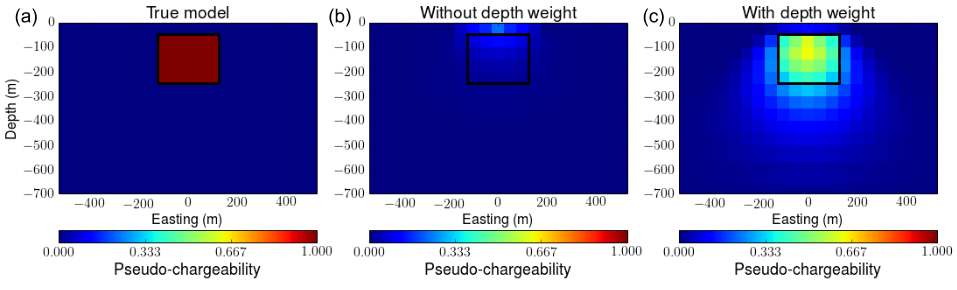
\includegraphics[width=1.\textwidth]{figures/Depthweight.png}
  \caption{Effect of depth weight in 3D IP inversion. (a) True pseudo-chargeability model on vertical section at 0 m-northing. Recovered pseudo-chargeability models (b) without depth weight and (c) with depth weight.}
  \label{F:Depthweight}
\end{figure}
\clearpage

%%% ===========================================================================
\subsubsection{Incorrect conductivity}
The background conductivity plays a central role our analysis. It is used in the EM decoupling process and it is also needed to compute the linearized sensitivities for inversion. Since we need to estimate this, usually through the inversion of EM survey data, it will never be correct. Here we explore some effects of an incorrect conductivity but  the consequences are problem dependent.

To observe the effects of an incorrect background we return to our conductive block in a halfspace. The estimated $dip$ data when the background is at the true value (xxx) as well as a factor of two too large (xxx) and a factor of two too small (xxx) are plotted in  along a survey line in Figure \ref{F:Reg_IPresp} 

We invert these three IP responses, and provide sections of the recovered pseudo-chargeability at 0m-northing. 
Figure \ref{F:Regional_IPInv}(a), (b) and (c) correspondingly show the recovered pseudo-chargeability from true, overestimated, and underestimated IP responses. 
With the true IP response, geometry of the IP body is reasonably recovered. 
Due to the negative residual field, the recovered pseudo-chargeability from the overestimated IP responses shows positive-valued artifacts near the IP body (Figure \ref{F:Regional_IPInv}(b)). 
In contrast, when the IP datum includes a positive residual field, we have negative-valued artifacts near the IP body (Figure \ref{F:Regional_IPInv}(c)) . 
Based on the definition of the  $w^e{t}$ and pseudo-chargeability and shown in equations \ref{eq: we} and \ref{eq: pseudochargeability}, the sign of the pseudo-chargeability should be positive. 
We can use this information as a positivity constraint in the inversion as shown in equation \ref{eq10}. 
Recovered pseudo-chargeability with this constraint for the underestimated case is shown in Figure \ref{F:Regional_IPInv}(d). 
Due to the positivity constraint, the inversion excludes to have negative values in the recovered pseudo-chargeability. 
Comparison of the observed and predicted data for this case shown in Figure \ref{F:Reg_obspred} clearly shows how this constraint prevents the fitting of positive residual fields originated from underestimated conductivity. We use the positivity  constraint for our following 3D IP inversion examples. 

The background conductivity is also needed when computing the sensitivity function, since we need the reference electric field, which is dependent on conductivity. 
An incorrect conductivity will have an effect on the sensitivity function as well. 
In order to test this effect, we compute the sensitivity  matrix using a half-space conductivity model ($\siginf = \sigma_1$). 
Figure \ref{F:True_vs_approx_sensitivity} compares the recovered pseudo-chargeability from the 3D IP inversion of the IP datum at 1.0 ms with the true and incorrect sensitivity function using half-space conductivity. 
There is not a large difference between the two inversions  which suggests that an approximate conductivity may still provide sensitivities that are adequate for inversion. This parallels results from EIP where even an approximate conductivity can still yield good results when inverting the data. There is some robustness in our sensitivity function with respect to an  incorrect conductivity. 
This implies that even we do not have 3D conductivity model, one can still apply our 3D IP inversion using half-space conductivity if the ATEM data includes distinctive IP response such as negative transients. 

\begin{figure}[htb]
  \centering
  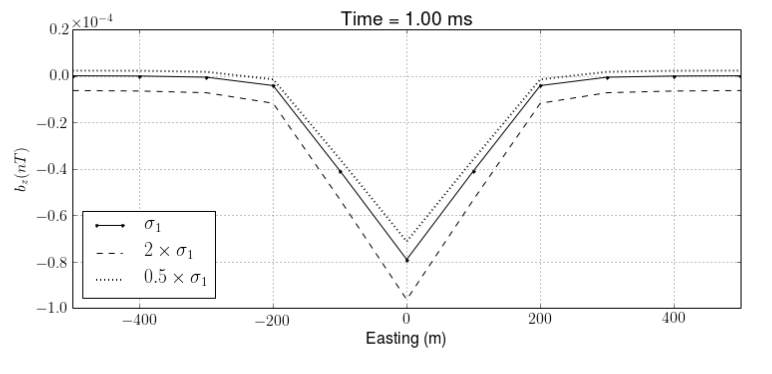
\includegraphics[width=1.\textwidth]{figures/Reg_IPresp.png}
  \caption{IP responses on a profile line at 0 m-northing.  IP responses are computed from perturbed $\siginf$ models. Half-space conductivity ($\sigma_1$) is perturbed two times higher or less resulting in overestimated (dotted line) and underestimated (dashed line) IP respones. Solid line shows the true IP response. }
  \label{F:Reg_IPresp}
\end{figure}

\begin{figure}[htb]
  \centering
  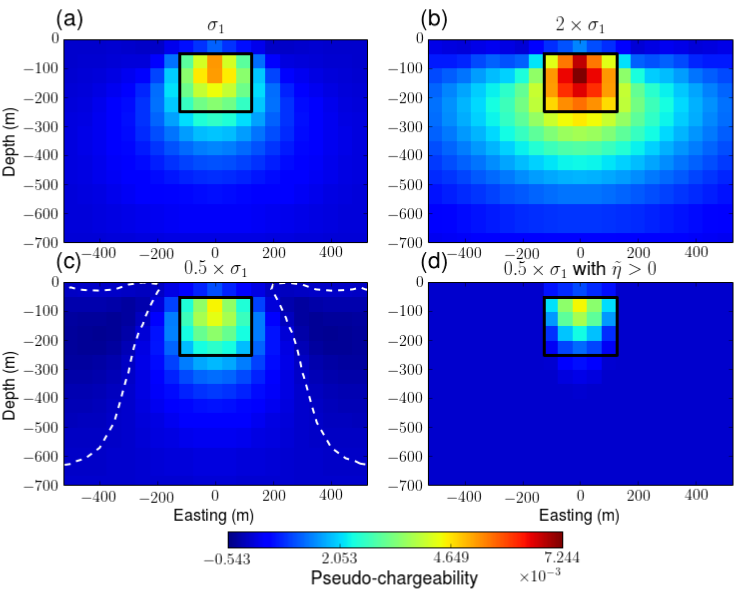
\includegraphics[width=1.\textwidth]{figures/Regional_IPInv.png}
  \caption{Recovered pseudo-chargeability sections from 3D IP inversions at 0 m-northing. (a) $\dip$ with true $\sigma_1$. (b) $\dip$ with 2$\times \sigma_1$. (c) $\dip$ with 0.5$\times \sigma_1$. (d) $\dip$ with 0.5$\times \sigma_1$ and the positivity constraint on the pseudo-chargeability.}
  \label{F:Regional_IPInv}
\end{figure}

\begin{figure}[htb]
  \centering
  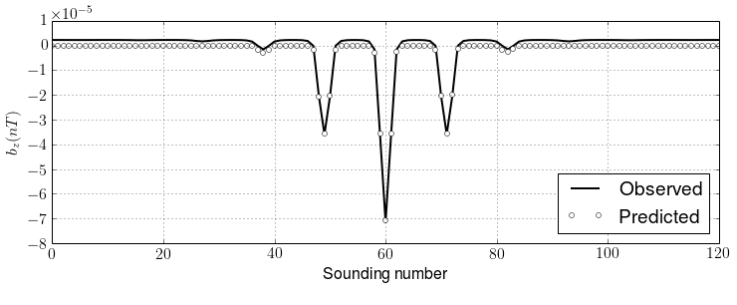
\includegraphics[width=1.\textwidth]{figures/Reg_obspred.png}
  \caption{Comparison of the observed (solid line) and predicted (empty circles) data. $\dip$ response was generated with underestimated half-space conductivity (0.5$\times \sigma_1$). The positivity constraint was used the 3D IP inversion.}
  \label{F:Reg_obspred}
\end{figure}

\begin{figure}[htb]
  \centering
  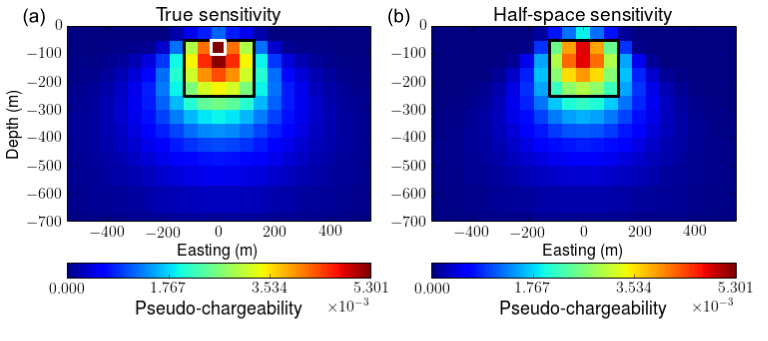
\includegraphics[width=1.\textwidth]{figures/True_vs_approx_sensitivity.png}
  \caption{Recovered pseudo-chargeabilty sections from the 3D IP inversions at 0m-northing.  (a) True and (b) incorrect $\siginf$ is used to compute sensitivity function. For the incorrect sensitivity we used half-space conductivity ($\sigma_1$).}
  \label{F:True_vs_approx_sensitivity}
\end{figure}
\clearpage
sssss

%%% ===========================================================================
\subsubsection{Extracting intrinsic IP parameters}
Although we recovered 3D pseudo-chargeability from the ATEM data, which provides distribution of chargeable bodies in the earth, still the pseudo-chargeability is not the intrinsic IP  parameters like the chargeability and time constant.
Fortunately, we have some possibility to recover this intrinsic IP information by interpreting multiple times of pseudo-chargeability together as we explained section \ref{section: extract_intrinsicIP}. 
We separately apply 3D IP inversion to the multiple channels of the IP datum ranging from 1-10 ms (14 channels), and recover pseudo-chargeability at those times. 
Here we choose true $\siginf$ model for both evaluation of IP datum and sensitivity function. 
To test the possibility of extracting intrinsic parameters from those recovered pseudo-chargeability at multiple times, we first choose a single pixel in the IP body shown in Figure \ref{F:IntrinsicIP}(a).  
This can be considered as the data for the inverse problem that we are going to solve to  estimate time constant ($\tau$) and chargeability ($\eta$) assuming $c$=1. 
A forward kernel for this inversion is shown in equation (\ref{eq: pseudochargeability_petaI}). 
% Seogi: need chage
% Averaged $w^e(t)$ from nine sounding locations chosen in Figure \ref{F:Equivalent_peta}(b) at the selected pixel of in the IP body is shown in Figure \ref{F:IntrinsicIP}(a).
The selected pixel is marked as white rectangle in Figure \ref{F:True_vs_approx_sensitivity}(a).  
Time decays of the observed and predicted data are shown in Figure \ref{F:IntrinsicIP}(b).
The estimated time constant ($\tau_{est}$) and chargeability ($\eta_{est}$) are 0.005 and 0.08, respectively. 
These are reasonable compared the those for true ones: 0.005 and 0.1, which suggests a potential to extract intrinsic IP parameters from ATEM data. 

\begin{figure}[htb]
  \centering
  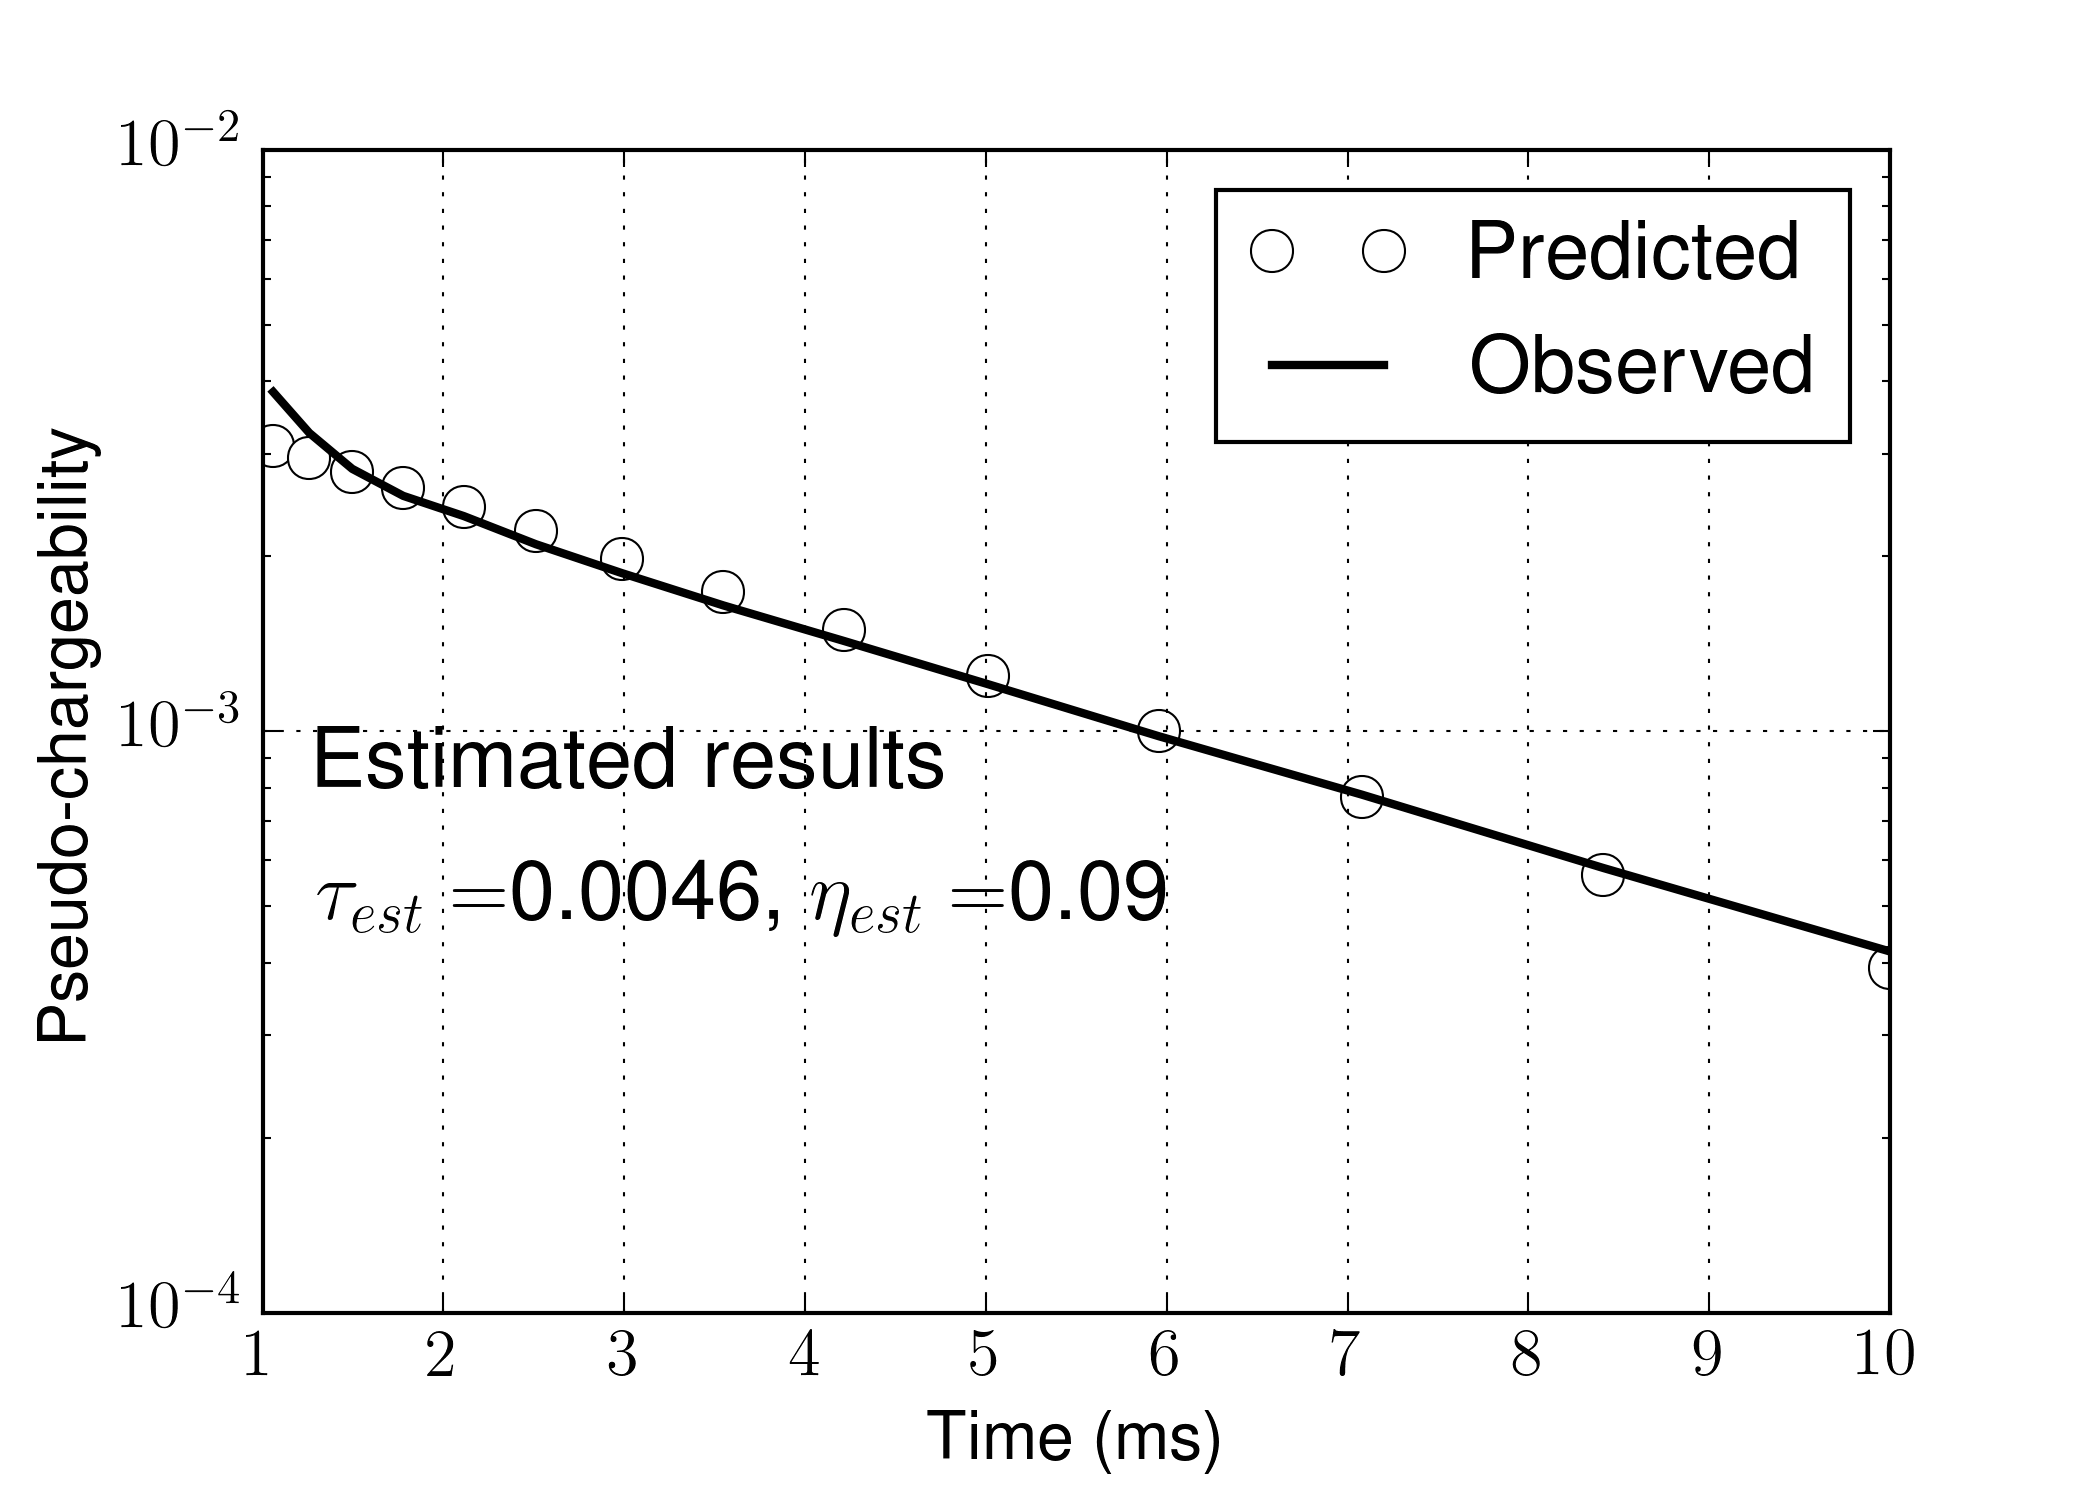
\includegraphics[width=1.\textwidth]{figures/IntrinsicIP.png}
  \caption{(a) The averaged $w^e(t)$ at the single pixel in the IP body (marked as white lines in \ref{F:True_vs_approx_sensitivity}(a). 
  (b) Comparisons of the observed (line) and predicted (empty circles) pseudo-chargeability at the same pixel. Estimated time constant and chargeability are expressed as $\tau_{est}$ and $\eta_{est}$, respectively.}
  \label{F:IntrinsicIP}
\end{figure}
\clearpage

% %% =============================================================================
% %% Section. Conclusions
% %% =============================================================================
% \section{Conclusions}
% In this paper, we have introduced an IP inversion procedure for the TEM data, especially for the inductive source. 
% This includes three main steps: 1) subtraction of the fundamental response from the observation, 2) linearization of the IP response as a function of the pseudo-chargeability, and 3) restoration of 3D pseudo-chargeability at multiple times, and further interpretation of the pseudo-chargeability to extract intrinsic IP parameters like Cole-Cole model. We used ATEM survey to test our IP inversion procedure.

% Assuming that we can recover reasonable 3D conductivity by inverting TEM data with exception of the IP-contaminated data, evaluation of the first step allows us to identify IP responses embedded in the observation. 
% By taking analogy from the EIP case, we effectively linearize ISIP response in time domain as a function of the pseudo-chargeability. 
% This pseudo-chargeability is defined as a fraction of the polarization current and the reference current, which may provide us the strength of the IP effect. 
% Different from the EIP case, the polarization charge buildup does not reach to the steady-state for the ISIP case due to the absence of steady-state electric field for inductive source. 
% This fundamental difference is carefully incorporated to the linearization with a proper choice of the reference electric field. 
% Numerical tests on the approximate IP current and responses demonstrated the capability of the linearized kernel for various conductivity structures: canonical, conductive, and resistive cases. 
% Our linearization is effective at certain late time when the IP effect is considerable to the EM effect, which may occur in the discharging phase. 

% In order to formulate 3D IP inversion, we suggested an equivalent pseudo-chargeability, which represents pseudo-chargeability of every transmitter, and tested with numerical simulation. 
% Based on this, we inverted IP responses at multiple times, separately, and recovered pseudo-chargeability at those times.
% Due to the possible lack of intrinsic depth resolution in our kernel for the ATEM survey, the depth weighting is used in the inversion.  
% Our 3D IP inversion recovered reasonable geometric shape and location of the chargeable body. 
% Because we may not recover true conductivity in practice, we tested possible effects of incorrect conductivity. 
% Two important places where we use conductivity are EM decoupling and sensitivity functions. 
% By designing two situations where we have postive or negative residual field in the IP response, we investigated the effect of incorrect conductivity in the IP response and the 3D IP inversion. 
% For the positive residual field, we showed that positivity constraint can be effectively used to prevent fitting those residual field. 
% In addition, even with a poor sensitivity function computed using half-space conductivity model, we recovered important information of the chargeable body such as geometric shape and location . 
% Finally, by interpreting recovered pseudo-chargeability at the center pixel of the IP body in time, we extracted Cole-Cole parameters: $\tau$ and $\eta$ by assuming $c=1$. 
% Estimated $\tau$ and $\eta$ were close to true ones, which indicates a potential to extract intrinsic IP parameters from the recovered pseudo-chargeability.  

% Our IP inversion procedure provides a framework that one can recover 3D distribution of the pseudo-chargeability, and possibly extraction of intrinsic IP parameters with post-processings of the pseudo-chargeability. 
% Because our inversion procedure requires 3D distribution of $\siginf$, which may not be trivial in some cases, this should be carefully investigated in the future for practical application of our inversion methodology. 
% In addition, our numerical examples was only treated the ATEM survey, even though application to different types of inductive source TEM survey such as Large-loop TEM may have different aspects that we need to consider. 
% However, still important items including EM decoupling, linearization and 3D IP inversion, which have been come up with and carefully tested in this study, will be fundamental backgrounds of following future studies about the ISIP in time domain. 

% =======================================================================
% SECTION (Appendix)
% =======================================================================

\section{Appendix}
%%% ===========================================================================
%%% SUBSECTION
\subsection{Discretization of steady-state Maxwell's equations}
\label{section:maxwell_discrete}
As shwon equation (\ref{eq: phiIPapprox_general}), computation of our linearized kernel requires solving steady-state Maxwell's equations. 
We discretize this system using mimetic finite volume (FV) method with weak formulation (\cite{Eldadbook}). 
For the discretization, we assume that the electric field $\e$ is discretized by grid function $\de$ on cell edges and magnetic flux density $\b$ is discretized by grid fuction $\db$ on cell faces. 
Electrical potential $\phi$ is discretized by grid fucntion  $\phi$ on cell nodes. For clear representation of the derivation, recall Maxwell's equations in steady state as
\begin{align}
  \j = \siginf\e = -\siginf\grad \phi, \\
  -\div \j = \div \j_s, \\
  \j\big|_{\partial \Omega}\cdot\hat{n} = 0,
  \label{eq:DCBCneumann}
\end{align}
where $\partial \Omega$ indicates boundary surface of the system and $\hat{n}$ is the normal vector of the boundary surface. Weak form of those equations can be written as
\begin{align}
  (\j, \vec{w}) + (\siginf \grad \phi, \vec{w}) = 0, \\
  -(\j, \grad \psi) = (\j_s, \grad \psi).
\end{align}
The inner products $(\j, \vec{w})$, $(\siginf \grad \phi, \vec{w})$,  $(\j, \grad \psi)$ and $(\j_s, \grad \psi)$ are edge based products. Here we define the inner product as
\begin{equation}
  (\vec{a}, \vec{b}) = \int_{\Omega} \vec{a}\cdot\vec{b} dv,
\end{equation}
where $\Omega$ is the volume of the system. By discretizing $\grad$ operator and the inner product in space, we obtain
\begin{equation}
  \Me\dj + \MeSigInf\dgrad\boldsymbol{\phi} = 0,
  \label{eq:DCdisceq1}
\end{equation}
\begin{equation}
  -\dgrad^T \Me\dj = \dgrad^T \Me\dj_s,
  \label{eq:DCdisceq2}
\end{equation}
where $\mathbf{M}^e_i$ is the mass matrices, which discretize the edge based inner product (\cite{Eldadbook}). This inner products are defined  as
\begin{align}
  \mathbf{M}^e_i = \diag(\Ace^T\diag(\vol)\mathbf{i}).
\end{align}
Here, $\mathbf{i}$ indicates a grid function on cell center like $\siginf$, and $\vol$ is the grid function for the cell volume. The averaging matrix $\Ace$ averages discrete function defined on the edges to the cell center. The mass matrix $\Me$ without subscript $i$ indicates that $\mathbf{i}$ is equal to the identity column vector of which all elements are one. By substituting equation (\ref{eq:DCdisceq1}) to (\ref{eq:DCdisceq2}), we have
\begin{equation}
  \A_{\siginf}\boldsymbol{\phi} = \mathbf{rhs}^{DC},
  \label{eq:DCdiscLin}
\end{equation}
where $\A_{\siginf} = \dgrad^T \MeSigInf\dgrad$ and $\mathbf{rhs}^{DC} = \dgrad^T \Me\dj_s$. 

%% ===========================================================================
%% SUBSECTION
\subsection{Discretization of the linearized kernel}
\label{section:linearkernel_discrete}
To obtain linear form of equation shown in equation (\ref{eq: dIP_lineareq}),
we first discretize Biot-Savart law shown in equations (\ref{eq: BiotbIP_approx}) and (\ref{eq: BiotbIPdt_approx}). In our discretization $\j^{IP}$ and  $\peta$ are defined on the cell center, and those for each time channel are constant in a cell volume, whereas $\eref$ is defined on the cell edges. 
We define the number of cells and edges in 3D space as nC and nE, respectively. Discretized IP current density, $\dj^{IP}_{cc} \in \mathbb{R}^{3nC}_{1}$, and defined on the cell center, since $\j^{IP}$ has three components, we first discretize integration operator including cross product ($\int_{v}\frac{ \times \hat{r}}{r^2}dv$) as
\begin{equation}
  \mathbf{G}_{Biot} =
  \begin{bmatrix}
       \mathbf{e}^T &  \mathbf{0}   & \mathbf{0}  \\
       \mathbf{0}   &  \mathbf{e}^T & \mathbf{0}  \\
       \mathbf{0}   &  \mathbf{0}   & \mathbf{e}^T
    \end{bmatrix}
  \begin{bmatrix}
       \mathbf{0}     &   \mathbf{S}_z   & -\mathbf{S}_y  \\
      -\mathbf{S}_z   &   \mathbf{0}     &  \mathbf{S}_x  \\
       \mathbf{S}_y   &  -\mathbf{S}_x   &  \mathbf{0}
    \end{bmatrix},
 \end{equation}
where
\begin{eqnarray*}
  \mathbf{S}_l =\diag(\mathbf{v}\oplus \mathbf{r}_l \oplus \frac{1}{\mathbf{r}^2}), \ l = x, \ y, \ z
\end{eqnarray*}
and the electric field, $\mathbf{e} \in \mathbb{R}^{nE}_1$ is a column vector, $\diag(\cdot)$ is the diagonal matrix and $\oplus$ is the Hadamard product. 
Then we discretize $\j^{IP}$ shown in equation (\ref{eq: jip_approx}) as
\begin{eqnarray}
  \dj^{IP}_{cc}(t) = \mathbf{S}\diag(\de^{F}_{max})\Ace^T\diag(\vol)\diag(\siginf)\peta(t),
\end{eqnarray}
where
\begin{eqnarray}
  \mathbf{S} = \mathbf{A}^{e}_{ccv}\Me^{-1}[\MeSigInf \mathbf{G} \A_{\siginf}^{-1}\mathbf{G}^T  - \mathbf{I}] \diag(\de^{F}_{max})\Ace^T\diag(\vol)\diag(\siginf).
\end{eqnarray}
and $\mathbf{A}^{e}_{ccv}$ is discrete averaging matrix from edge to cell center with consideration of three component vector: $\in \mathbb{R}^{3nC}_{nE}$. 
Thus, we can have linear equation for $k^{th}$ time channel as
\begin{eqnarray*}
  \db^{IP}_i = \Gbiot \mathbf{S} \peta_i,
\end{eqnarray*}
where subscript $i$ indcates $i^{th}$ time channel. Finally, by letting
\begin{equation}
  \mathbf{J} = -\Gbiot\mathbf{S},
  \label{eq: Sense}
\end{equation}
we have
\begin{eqnarray}
  \db^{IP}_i = \mathbf{J}\peta_i,
  \label{eq: bIP_linear}
\end{eqnarray}
where $\mathbf{J}$ is the Jacobian matrix of the linear equation, and since $\mathbf{J}$ is static, we also obtain
\begin{eqnarray}
  -\frac{\partial\db^{IP}}{\partial t}\Big|_i = \mathbf{J}(-\frac{\partial \peta}{\partial t}\Big|_i).
  \label{eq: dbIPdt_linear}
\end{eqnarray}

% \subsection{Discrete Helmholtz decomposition}
% \label{section:helmholtz}
% In continuous space, we can decompse arbitrary vector field as 
% \begin{equation}
%   \e = -\grad\phi -\vec{a},
% \end{equation}
% where $\div \vec{a} = 0$. 
% Decomposition of discrete electric field, $\de$, can be expressed as
% \begin{equation}
%   \Me\de = -\Me\dgrad \boldsymbol{\phi} -\Me\mathbf{a},
% \end{equation}
% where $\boldsymbol{\phi}$ and $\mathbf{a}$ are discrete scalar and vector potentials, respectively. 
% By taking discrete divergece ($-\dgrad^T$), we obtain
% \begin{equation}
%   -\dgrad^T\Me\dgrad\boldsymbol{\phi} = \dgrad^T\Me\mathbf{a} + \dgrad^T\Me\de
% \end{equation}
% Since the vector potential $\vec{a}$ is divergece free, the first term in the right-hand side is zero. Thus, we obtain
% \begin{equation}
%   \dgrad^T\Me\dgrad\boldsymbol{\phi} = -\dgrad^T\Me\de. 
% \end{equation}
% By solving this linear system we can first compute $\boldsymbol{\phi}$, then by subtracting this from $\de$, we can also obtain the vector potental, $\mathbf{a}$. 
% %% Appendix
% 1. Discretization of the linearized kernel
% 2. Numerical evaluation of the Helmholtz decomposition

\bibliographystyle{plain}
\bibliography{reference}

\end{document}



